% === No modificar éstos parámetros === 
\documentclass[12pt,letterpaper]{article}     % Tipo de documento y otras especificaciones
\usepackage[utf8]{inputenc}           % Para escribir tildes y eñes
\usepackage[spanish]{babel}                   % Para que los títulos de figuras, tablas y otros estén en español
\usepackage{mdwlist}
\usepackage{multirow}
\addto\captionsspanish{\renewcommand{\tablename}{Tabla}}					% Cambiar nombre a tablas
\addto\captionsspanish{\renewcommand{\listtablename}{Índice de tablas}}		% Cambiar nombre a lista de tablas
\usepackage{geometry}
\usepackage{lipsum}
\geometry{left=30mm,right=30mm,top=25mm,bottomhttps://www.overleaf.com/project/5d682739555c82408dd28ba3=25mm} % Tamaño del área de escritura de la página

\usepackage{ucs}
\usepackage{amsmath}      % Los paquetes ams son desarrollados por la American Mathematical Society
\usepackage{amsfonts}     % y mejoran la escritura de fórmulas y símbolos matemáticos.
\usepackage{amssymb}
\usepackage{graphicx}     % Para insertar gráficas
\usepackage[lofdepth,lotdepth]{subfig}	% Para colocar varias figuras
\usepackage{unitsdef}	  % Para la presentación correcta de unidades
\renewcommand{\unitvaluesep}{\hspace*{4pt}}	% Redimensionamiento del espacio entre magnitud y unidad
\usepackage[colorlinks=true,urlcolor=blue,linkcolor=black,citecolor=green]{hyperref}
\usepackage{float}
\usepackage{booktabs}
\batchmode
\bibliographystyle{plain}
\pagestyle{plain}
\usepackage{pdfpages}
\pagenumbering{arabic}
\usepackage{lastpage}
\usepackage{fancyhdr}	% Para manejar los encabezados y pies de página
\usepackage{adjustbox}
\pagestyle{fancy}		% Contenido de los encabezados y pies de pagina
\usepackage{matlab}
%%%%%%%%%%%%%%%%%%%%%%%%%%%%%%%%%%%%%%%%%%%%%%%%%%%%%%%%%%%%%%%%%%%%%%%
\usepackage{pdfpages}


\usepackage{lastpage}
\usepackage{fancyhdr}	% Para manejar los encabezados y pies de página
\pagestyle{fancy}		% Contenido de los encabezados y pies de pagina
\usepackage{multicol}
%\usepackage{subfigure}
\usepackage{textcomp}
\usepackage{amsfonts}     % y mejoran la escritura de fórmulas y símbolos matemáticos.
%%%%%%%%%%%%%%%%%%%%%%%%%%%%%%%%%%%%%%%%%%%%%%%%%%%%%%%%%%%%%%%%%%%%%%%%%%%%%%%%%%%%%%%%%%%%%%%%%%%%%%%%%%%%%%%%%%%%%%%%%%%%%%%%%%

\lhead{IE0409 - Análisis de Sistemas}
\chead{}
\rhead{Proyecto Final}


\lfoot{Escuela de Ingeniería Eléctrica}
\cfoot{\thepage\ }
\rfoot{Universidad de Costa Rica}
\usepackage{enumerate}
\usepackage{enumitem}

%%%%%%%%%%%%%%%%%%%%%%%%%%%%%%%%%%%%%%%%%%%%%%%%%%%%%%%%%%%%%%%%%
\begin{document}
% Hoja de portada, únicamente editar nombres y códigos

\begin{titlepage}
	\centering
	
\includegraphics[width=0.5\textwidth]{Imagines/logo_ucr.png}\par\vspace{1cm}
	{\scshape\LARGE Universidad de Costa Rica \par}
	\vspace{0.5cm}
	{\scshape\Large Análisis de Sistemas \par}
	\vspace{.2cm}
    {\scshape\Large IE0409 \par}
	\vspace{1cm}
	{\Large\bfseries Proyecto final: Intercambiador de calor (Avance I)\par}
	\vspace{1cm}
    {\itshape Miguel Ángel Díaz Galeano, B12234 \par}
    {\itshape Daniel Alvarado Hernández, A90283 \par}
    {\itshape Luis Alvarado Matarrita, 880166      \par}
    {\itshape       \par}
    
    
	\vfill
    Grupo de clase: 03 \par
    Grupo de trabajo: 08 \par
	Prof. Joaquín Cordero Cordero
	\vfill
	{Fecha de entrega: 06/10/19}
\end{titlepage}
%%%%%%%%%%%%%%%%%%%%%%%%%%%%%%%%%%%%%%%%%%%%%%%%%%%%%%%%%%%%%%%%%

\section*{Resumen}
En el presente escrito se detalla el modelado de un intercambiador de calor. Para la realización del proyecto se realiza una recopilación de aspectos teóricos importantes que rodean el tema abordado. Se mencionan los diferentes tipos de intercambiadores presentes en la industria según su método de funcionamiento.
Se desarrolla un marco físico-matemático basado en los principios físicos relevantes en la transferencia del calor. 
Se determinan los modelos, parámetros y variables de estados relevantes y a utilizar en la simulación del sistema a través de MATLAB y Simulink.
Se interpreta el comportamiento del sistema a través de los resultados de la simulación y se derivan las conclusiones de la investigación. \\
\par
\begin{small}
\textbf{Palabras claves}: \textit{intercambiador, calor, transferencia, convección, conducción, radiación, energía, térmico, enfriamiento, termodinámica }
\end{small}

\newpage
\let\OLDthebibliography=\thebibliography
\def\thebibliography#1{\OLDthebibliography{#1}%
\addcontentsline{toc}{section}{\refname}}


\makeatletter
\renewcommand\@biblabel[1]{#1. \ }
\makeatother


%%%%%%%%%%%%%%%%%%%%%%%%%%%%%%%%%%%%%%%%%%%%%%%%%%%%%%%%%%%%%%%%%
%Palabras claves

\setcounter{page}{1}
\pagenumbering{Roman}
\tableofcontents

\newpage

\listoffigures
\newpage
\listoftables

\newpage

\section*{Nomenclatura}

\begin{description}[labelindent=1cm,labelwidth=2.25cm,align=left]
\item [${ q }$]  Velocidad de flujo de calor
\item [$Q$] Flujo de calor
\item [$T$] Temperatura
\item [$A$] Área
\item [$L$] Ancho
\item [$G$]  Irradiación
\item [$J$] Reflexión de radiación
\item [${  \sigma }$]  Constante de Stefan-Boltzmann
\item [${ E }_{ b }$] Potencia del cuerpo negro
\item [$\epsilon$] Emisividad
\item [$\alpha$] Absorbancia
\item [${ Re }$] Número de Reynolds
\item [${ h }_{ c }$] Coeficiente de transferencia de calor por convección
\item [${Nu }$]  Número de Nusselt
\item [$Pr$] Número de Prandtl
\item [${ D}_{h }$] Diámetro hidráulico
\item [${ m }$] Flujo neto de la masa
\item [${ \rho}$] Densidad del liquido
\item [${ V }$] Volumen del intercambiador
\item [${ T(t) }$] Temperatura del líquido en el intercambiador
\item [${ T_i (t) }$] Temperatura del flujo que entra al tanque
\item [${ T_s(t) }$] Temperatura del líquido en el serpentín
\item [${ \lambda }$] Flujo de corriente del líquido
\item [${ w(t) }$] Flujo del vapor
\item [${ C_M }$] Capacidad calórica del metal del serpentín
\item [${ C_V }$] Capacidad calórica del líquido en el intercambiador
\item [${ C_p }$] Capacidad calórica de la masa que se quiere calentar






\end{description}

%
\newpage
%
\pagenumbering{arabic}
\setcounter{page}{1}
%%%%%%%%%%%%%%%%%%%%%%%%%%%%%%%%%%%%%%%%%%%%%%%%%%%%%%%%%%%%%%%

%%%%%%%%%%%%%%%%%%%%%%%%%%%%%%%%%%%%%%%%%%%%%%%%%%%%%%%%%%%%%%%%%%
\section{Introducción}  
La ciencia de la transfencia de calor estudia, analiza y modela la rapidez o razón de transferencia de calor, además que éstos son temas fundamentales en la ingeniería.
Desde el punto de vista de la termodinámica y los parámetros citados supra, la transferencia de calor reciben un enfoque en cuanto a los mecanismos de propagación del calor: convección, radiación y conducción las cuales requieren de interacción entre las distintas sustancias.
\begin{itemize}
\item Conducción:
Se dá entre superficies sólida y líquidas o sólidas que registran movimiento que junto con la conducción originan este tipo de transferencia.

\item Convección:
Consiste en la transferencia entre partículas energitizadas hacia otros de menor energía (Calor).


\item Radiación:
Energía que emite una fuente como resultado de modificaciones en la estructura electrónica. Dicha energía es liberada en forma de ondas electromagnéticas (fotones).

\end{itemize}
El meollo de los problemas cientificos está en la obtención de ecuaciones que describen y relacionan las variables que involucran; ecuaciones que conllevan a formulaciones matemáticas que precisan infinitesionalmente dichas relaciones.
Los modelos  obtenidos son importantes debido a que anticipan distintas posibles soluciones a los problemas y tomar las mejores decisiones.

La transferencia de calor se explica mediante teoría y modelos. Las variables involucradas en esas teorías responden a modelos generales que hacen referencia a entradas, memoria y salida.

El presente trabajo consiste en el análisis de variables seleccionadas bajo un escenario específico con el fin de determinar las relaciones entre dichos parámetros, según los postulados teóricos vistos en clase.

Particulamente el enfoque del trabajo es el análisis número para aproximar las ecuaciones y el modelo en variables de estado del intercambio de calor de una pared plana.


\subsection{Alcances}
Este trabajo permite conocer y entender el proceso del modelado y simulación de un intercambiador de calor, desde su esencia teórica descrito en los fundamentos de funcionamiento físicos hasta el modelado matemático que permite simularlo. Se ilustra el conocimiento necesario del uso de software propietario MATLAB\circledR\space  y SIMULINK\circledR\space para la parte de simulación.
\newpage
%%%%%%%%%%%%%%%%%%%%%%%%%%%%%%%%%%%%%%%%%%%%%%%%%%%%%%%%%%%%%%%%%%
\newpage
\subsection{Objetivos}
\subsubsection{Objetivo General}
Modelar matemáticamente y simular por medio de software un sistema basado en una aplicación real en la industria tal como lo son los intercambiadores de calor.

\subsubsection{Objetivos Específicos}
\begin{itemize}
\item Exponer los fundamentos físicos principales presentes en el los principios de funcionamiento del intercambiador de calor.
\item Investigar por medio recursos bibiográficos sobre los antecedentes y avances a través del tiempo para las aplicaciones de los intercambiadores de calor.
\end{itemize}
\begin{itemize}
\item Aplicar los conocimientos adquiridos en el curso de análisis de sistemas I para la construcción del modelo matemático y su simulación en MATLAB.
\end{itemize}

\subsection{Metodología}
Para el desarrollo del trabajo se incluyeron  los siguientes pasos y procedimientos:

\begin{itemize}

\item Recopilación bibliográfica cuyo contenido aborde el tema del intercambiador de calor para ampliar el conocimiento sobre el tema y el desarrollo de este trabajo.
\item Incorporación al trabajo de toda la teoría que facilite el desarrollo del modelo matemático y físico de un intercambiador de calor. 
\item Utilización de herramientas de simulación MATLAB/Simulink, para el modelado y simulación de sistemas.
\item Análisis en el tiempo y en la frecuencia del sistema desarrollado, junto con todas las conclusiones que se deriven de las simulaciones realizadas a lo largo de este documento.
 
 \end{itemize}



%%%%%%%%%%%%%%%%%%%%%%%%%%%%%%%%%%%%%%%%%%%%%%%%%%%%%%%%%%%%%%%%%
\newpage

\section{Marco Teórico}

\subsection{Antecedentes históricos}
El calor como concepto ha cambiado a través del tiempo, Francis Bacon (1561-1626) menciona al calor en su libro "Novus Organum", tabulando las que el consideraba como fuentes de calor, entre ellas: la luz, los rayos e incluso algunas hierbas aromáticas o especias que causaban "una sensación de calor cuando eran digeridas".
Pierre Gassendi (1592-1655), veía al calor y al frío como diferentes especies de materia, y consideraba al frío como átomos que penetraban los líquidos y los solidificaba de alguna manera.
En un avance importante para la termodinámica, Joseph Black (1728-1799) derrite hielo muy lentamente y nota que la temperatura del agua no cambia. Así se empieza a distinguir las propiedades de \textit{cantidad} e \textit{intensidad} del calor. La segunda cuantificada con la temperatura. 
Antoine Lavoisier (1743-1794) enlista al calor como un elemento de la materia y lo consideraba un fluido que llamó \textit{calórico}. \cite[p.\ 27]{Cengel}
Benjamin Thompson (1753-1814), desacredita la teoría calórica, y menciona que existe un vínculo entre el movimiento y el calor.
James Prescott Joules (1818-1889) finalmente establece un vínculo directo entre el movimiento y el calor, y utiliza conceptos de energía y trabajo para explicar la cantidad necesaria para aumentar un grado Fahrenheit a una libra de agua.


El intercambiador de calor de placas apareció en la década de 1920, en un aporte y se aplicó a la industria alimentaria, sucesivamente continúo el desarrollo hasta que en los años 60s, debido al avance tecnológico con mayor necesidad de gestionar el calor, la termometría toma mayor auge.\\
Posteriormente, los nuevos retos de mayor eficiencia en este campo  aunado a la necesidad de ahorro energético conllevan al desarrollo de dispositivo cada vez más compactos y eficientes. 
4


\subsection{Intercambiadores de Calor}

Existen sistemas en diversas áreas de la ingeniería, ya sean químicos, mecánicos, nucleares u otros, que requieren transferencia de calor de un lugar a otro durante su operación.  Los intercambiadores de calor son aparatos que facilitan el intercambio de calor entre dos fluidos que se encuentran a temperaturas diferentes y evitan al mismo tiempo que se mezclen entre sí.  \cite[p.\ 269]{Cengel}
Estos varían en tamaño y diseños que se ajustan a las necesidades particulares.
En este sentido los intercambiadores de calor se pueden catalogar según su construcción como:


\begin{itemize}
\item \textbf{Tubos y coraza:} Muy común en aplicaciones industriales. Consiste en gran cantidad de tubos dentro de una coraza o armazón, los fluidos circulan tanto por el tubo como por el espacio entre éste y la armazón. Este tipo de intercambiador se fabrica en distintos diseños que se distinguen por la dirección de los fluidos o diseños en su estructura que buscan mayor contacto e intercambio de calor. La figura \ref{fig:coraza} ilustra este tipo de regenerador.
\end{itemize}


\begin{figure}[H]
\centering
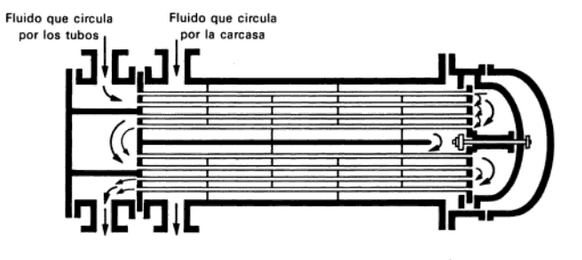
\includegraphics[width=0.7\textwidth]{coraza.jpg}
\caption{Intercambiador de tubos y coraza \cite{Lopez} (p.58)}
\label{fig:coraza}
\end{figure}

\begin{itemize}
\item \textbf{Plato:} El intercambiador de calor de tipo plato, como se muestra en la figura \ref{fig:plato}, consiste de placas en lugar de tubos para separar a los fluidos caliente y frío. Estos se alternan entre cada una de las placas y  el flujo del líquido es direccionado entre las placas. Ya que cada una de las placas tiene un área superficial muy grande, las placas proveen un área extremadamente grande de transferencia de térmica a cada uno de los líquidos. Esto hace al intercambiador de placa capaz de transferir mucho más calor con respecto a un intercambiador de tubos y coraza con volumen semejante, esto es debido a que las placas proporcionan una mayor área que la de los tubos. Por lo tanto es mucho más pequeño que el de carcaza y tubos para la misma capacidad de intercambio de calor.\textbf{}
\end{itemize}

\begin{figure}[H]
\centering
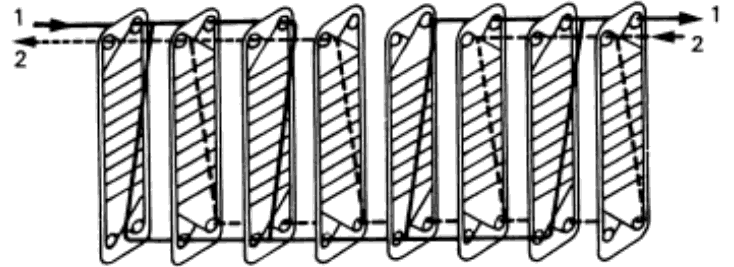
\includegraphics[width=0.7\textwidth]{placas.PNG}
\caption{Intercambiador de placas \cite{Lopez} (p.59)}
\label{fig:plato}
\end{figure}

Según Jaramillo (2007), los intercambiadores de placa o plato no se utilizan extensamente debido a la inhabilidad de sellar confíablemente las juntas entre cada una de las placas. Debido a este problema, el tipo intercambiador de la placa se ha utilizado solamente para aplicaciones donde la presión es pequeña o no muy alta, por ejemplo en los refrigeradoresde aceite para máquinas. Actualmente se cuentan importantes avances que han mejorado el diseño de las juntas y sellos, así como el diseño total del intercambiador de placa, esto ha permitido algunos usos a gran escala de este tipode intercambiador de calor. Así, es más común que cuando se renuevan viejas instalaciones o se construyen nuevasinstalaciones el intercambiador de la placa está substituyendo paulatinamente a los intercambiadores de carcaza y tubo.

Adicionalmente los intercambiadores de calor se pueden clasificar según su modo de operación, los principales siendo los de flujo paralelo, contraflujo y flujo cruzado.

\begin{itemize}
\item \textbf{Flujo paralelo}: Como se esquematiza en la figura \ref{fig:paralelo}, hay un flujo paralelo cuando el flujo interno (en los tubos) y el flujo externo (de la carcaza) ambos fluyen en la misma dirección. En el caso de un flujo paralelo, los dos fluidos entran al intercambiador por el mismo extremo y estos presentan una diferencia de temperatura notable. Como el calor se transfiere del fluido con mayor temperatura hacia el fluido de menor temperatura se llegará a una temperatura intermedia en el flujo de salida por equilibrio térmico lo que significa que el fluido refrigerante o de menor temperatura aumentará. Es importante dejar claro que el fluido con menor temperatura nunca alcanza la temperatura del fluido más caliente.
\end{itemize}

\begin{figure}[H]
\centering
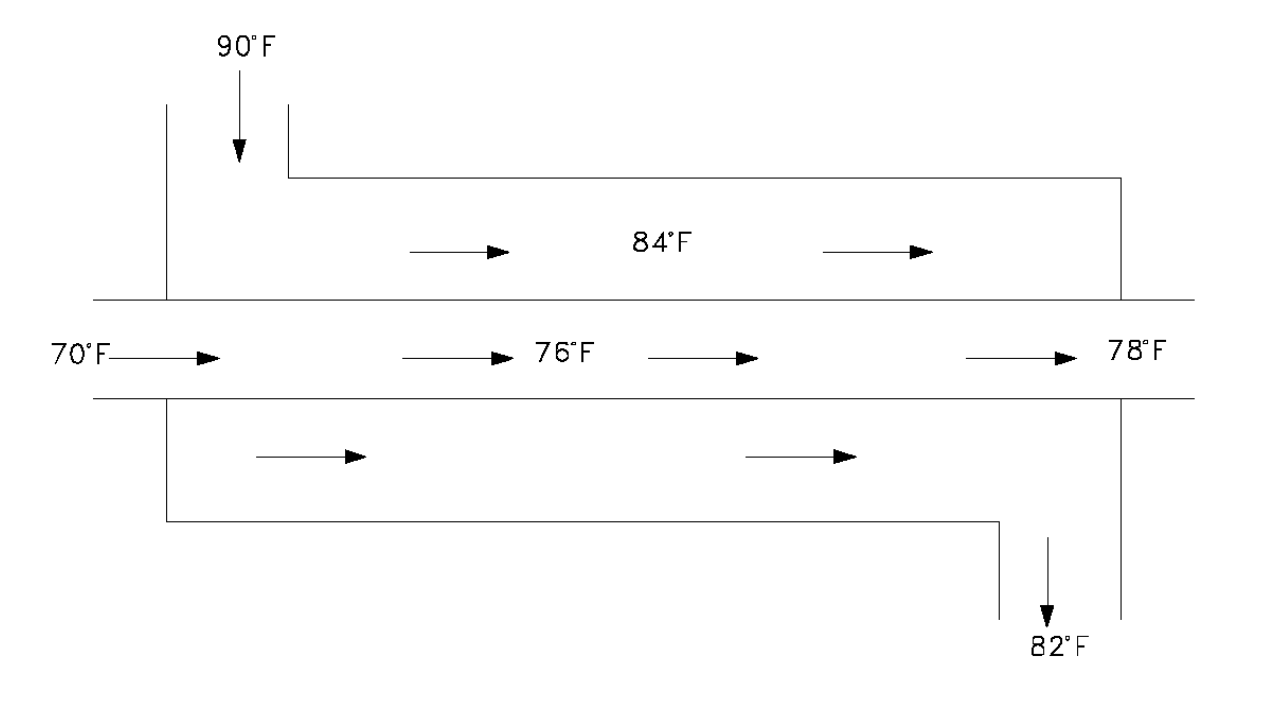
\includegraphics[width=0.7\textwidth]{paralelo.PNG}
\caption{Flujo paralelo. [Tomado de \cite{Jaramillo}]}
\label{fig:paralelo}
\end{figure}

\begin{itemize}
\item \textbf{Contraflujo}: Un contraflujo se da cuando los dos fluidos fluyen paralelamente pero en sentido opuesto. Cada uno de los flujos entra al intercambiador por diferentes extremos. A diferencia con el intercambiador de calor de flujo paralelo, el intercambiador de contraflujo puede presentar la temperatura más alta en el fluido refrigerante y la temperatura más baja en el fluido caliente después de realizada la transferencia de calor. Este comportamiento se ilustra en la figura \ref{fig:contraflujo}.
\end{itemize}

\begin{figure}[H]
\centering
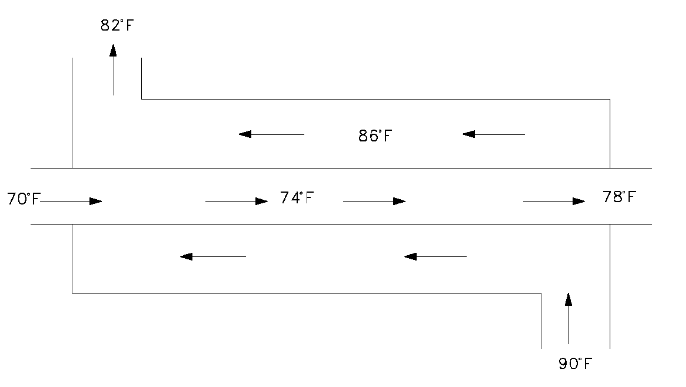
\includegraphics[width=0.7\textwidth]{contraflujo.png}
\caption{Contraflujo. [Tomado de \cite{Jaramillo}]}
\label{fig:contraflujo}
\end{figure}

\begin{itemize}
\item \textbf{Flujo cruzado}: En el flujo cruzado, ver figura \ref{fig:flujocruz}, uno de los fluidos fluye perpendicular al otro. Es decir, uno de los fluidos atraviesa los tubos mientras que el otro pasa alrededor de estos formando un ángulo de de noventa grados. Este tipo de intercambiador de calor son comúnmente utilizados donde uno de los fluidos presenta cambio de fase y por tanto se tiene un fluido pasando por el intercambiador en dos fases o bifásico (Jaramillo, 2007). Un ejemplo típico de este tipo de intercambiador es en los sistemas de condensación de vapor.
\end{itemize}

\begin{figure}[H]
\centering
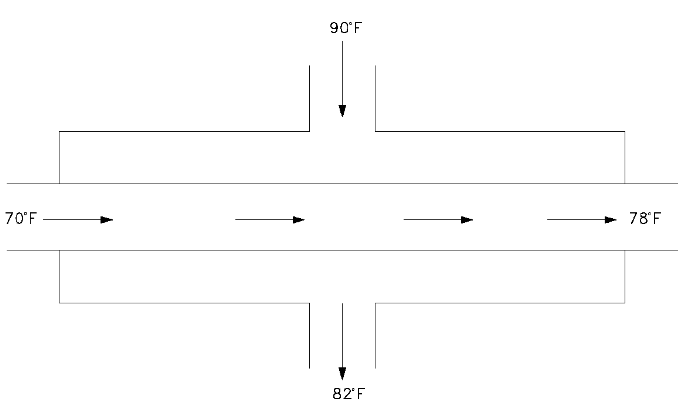
\includegraphics[width=0.7\textwidth]{flujocruz.png}
\caption{Flujo cruzado. [Tomado de \cite{Jaramillo}]}
\label{fig:flujocruz}
\end{figure}

En la actualidad, la mayoría de los intercambiadores de calor no son puramente de flujo paralelo, contraflujo, o flujo cruzado; estos son comúnmente una combinación de los dos o tres tipos de intercambiador. (Jaramillo, 2017)

Otros calificativos comunes de los intercambiadores de calor son los de un sólo paso o de múltiples pasos y los intercambiadores regenerativos:



%\item  \textbf{Compactos: }La superficie expuesta es muy grandes respecto a su volumen y comunmente los fluidos circulan de manera perpendicular. La Figura \ref{fig:Compacto} muestra un ejemplo de dispositivo de este tipo.


%\begin{figure}[H]
%\centering
%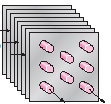
\includegraphics[width=0.3\textwidth]{Compacto.png}
%\caption{Intercambiador compacto de gas hacia líquido \cite{Cengel} (p.954)}
%\label{fig:Compacto}
%\end{figure}

%\begin{itemize}
  
  
%\item \textbf{Tubos concéntricos} Los fluidos calientes y fríos circulan por conductos distinto ya sea en la misma dirección (Flujo paralelo) o en direcciones opuestas (Contraflujo); la figura \ref{fig:Flujo en tubos} hace referencia a un diseño particular de tubos - coraza.

%\begin{figure}[H]
%\centering
%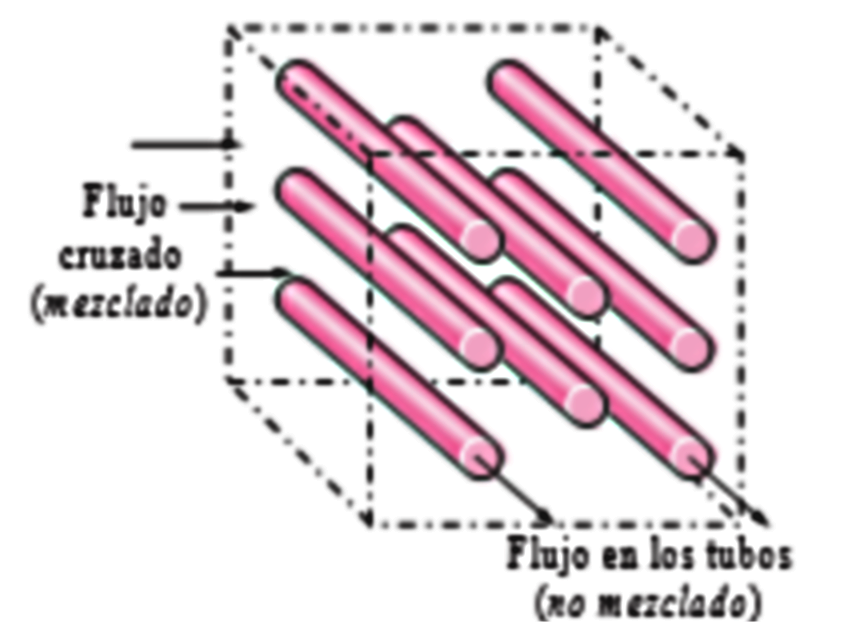
\includegraphics[width=0.5\textwidth]{Flujo_Cruzado-nuevo.png}
%\caption{Flujo en tubos \cite{Cengel} (p.954)]}
%\label{fig:Flujo en tubos}
%\end{figure}

\begin{itemize}
\item \textbf{De paso simple o múltiples pasos:} Se catalogan de esta manera según el número de veces por las que se pasan los dos fluidos por el intercambiador, siendo los de múltiples pasos los que intercambian el calor más de una vez. En la figura \ref{fig:pasos} se contrastan estos tipos de intercambiadores.
\end{itemize}

\begin{figure}[H]
\centering
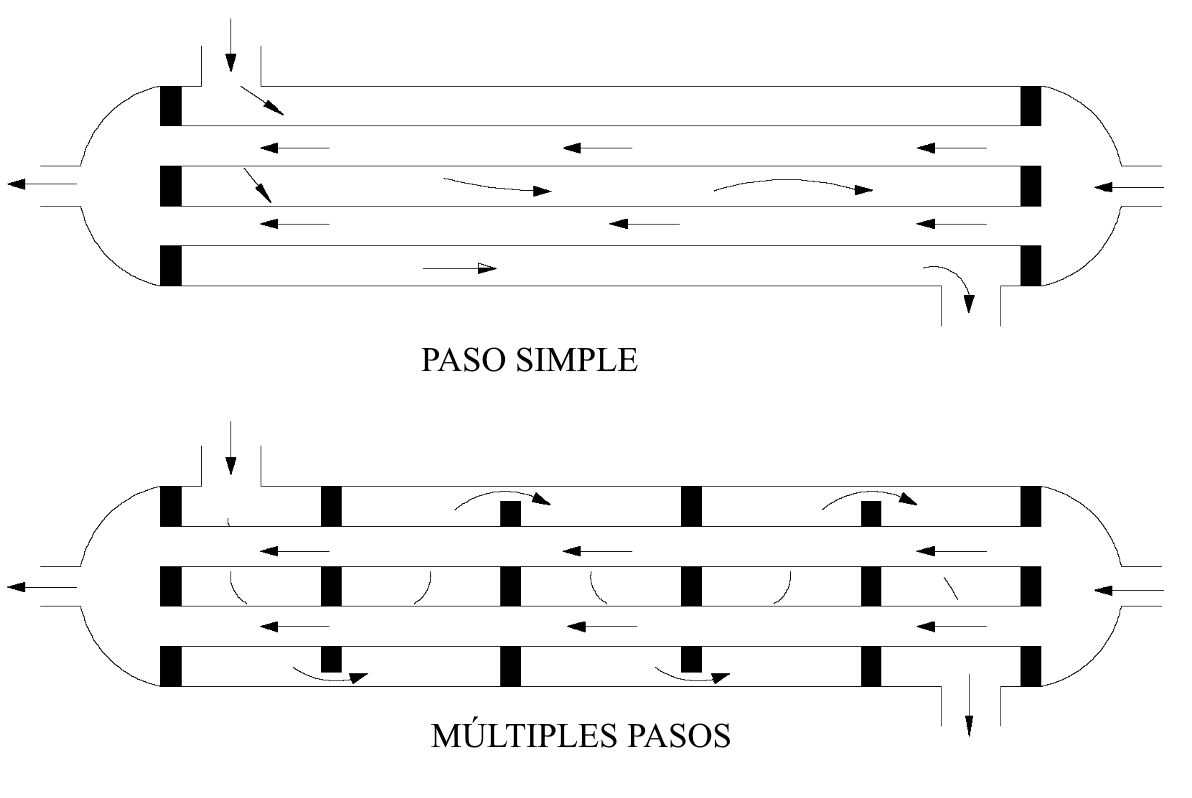
\includegraphics[width=0.7\textwidth]{pasos.png}
\caption{Comparación esquemático de un intercambiador de paso simple con uno de múltiples pasos \cite{Jaramillo}}
\label{fig:pasos}
\end{figure}

\begin{itemize}
\item \textbf{Regenerativo:} Un intercambiador regenerativo aprovecha la energía (calor) del fluido caliente y la almacena, por lo general en un "lecho de sólidos"\ con una apreciable capacidad de almacenamiento calórico. Estos sólidos se calientan de forma gradual, pero antes de llegar al equilibrio los flujos son cambiados y entonces el fluído frío remueve el calor del lecho. Es un tipo de sistema en realimentación. 
\end{itemize}


\subsection{Fundamentos de transferencia de calor}

\subsubsection{Temperatura y energía interna}
 
Según el autor Eduardo, la energía interna, dado que es una función de estado, está relacionada con los parámetros termodinámicos del sistema (presión, temperatura y composición) y puede calcularse a partir de ellos. Cuando la composición del sistema permanece sin cambios, la energía interna es función de la presión y la temperatura.

Por lo general, los cambios en la energía interna con presión no son significativos siempre que estos cambios de presión no produzcan cambios de fase en el sistema, por lo que la energía interna a veces puede considerarse una función exclusiva de la temperatura. Es por eso que a veces se usa el término energía térmica. Esta expresión, aunque no tiene un significado termodinámico preciso, es gráfica e intuitiva.

La energía interna se almacena en un sistema a nivel molecular o atómico. Esto significa que los átomos o moléculas pueden existir en diferentes niveles de energía, que corresponden, por ejemplo, a diferentes velocidades o frecuencias de sus movimientos u oscilaciones.

La temperatura es el observable macroscópico que está más directamente relacionado con estos niveles de energía. Así, las moléculas o átomos con más energía se observan como más " calientes". Por ejemplo, en el caso de los gases monoatómicos, la energía cinética de la molécula está relacionada con la temperatura mediante la expresión.\cite[p.2-3]{Eduardo} 

\begin{equation}
   \frac {mu^2 }{2} =\frac {3kT }{2}  
    \label{eq:temperature.internalenergy}
\end{equation}

\subsubsection{Relación entre termodinámica y transferencia de calor}

\cite[p\ 4]{Mills} La transferencia de calor en ingeniería se ocupa del cálculo de la velocidad a la que el valor fluye en un medio dado,a través de una interfaz o entre dos superficies,así como de la determinación de las temperaturas dadas.Es importante entender la diferencia esencial entre transferencia de calor en la ingeniería y lo que usualmente se llama termodinámica. La termodinámca clásica aborda sistemas en equilibrio. Su metodología puede usarse para calcular la energía necesaria para llevar a un sistema de un estado de equilibrio a otro, pero no permite determinar la velocidad a la que ocurre el cambio.

\subsubsection{Calor y la Primera ley de la termodinámica}

 \cite[p\ 2-2]{Eduardo} El calor se puede definir como la energía que se transfiere debido a la existencia de una diferencia de temperatura entre dos sistemas o entre dos partes de un sistema. Cuando hablamos de calor, siempre nos referimos a energía en tránsito. No se puede decir que un sistema acumula calor. El calor se transfiere a un sistema, y una vez que ingresa al sistema, esta energía se transforma en otros tipos de energía, como la energía cinética o interna o el trabajo mecánico.

\cite[p\ 4]{Mills} En particular, se aplica la primera ley de la termodinámica, generalmente en formas muy sencillas, puesto que los efectos de trabajo a menudo puede despreciarse. La primera ley es una manera de enunciar el principio de la conservación de la energía,que es una de las leyes fundamentales de la física. En transferencia de calor, con frecuencia nos referimos a la primera ley como el principio de conservación de la energía,o simplemente como balance de calor o energía cuando no se realiza trabajo.


En un sistema cerrado se tiene un volumen V $[m^3]$ y una densidad $[\frac{kg}{m^3}]$. Se transfiere calor al sistema a una velocidad $\dot{Q}  [\frac{J}{s} o W]$

\begin{equation}
\Delta{U} = \dot{Q}\Delta t + \dot{Qv}\Delta t     
\label{eq:varenergiainterna}
\end{equation}

\begin{equation}
\frac{\Delta{U}}{\Delta t} = \dot{Q} + \dot{Qv}    
\label{eq:varenergiainterna2}
\end{equation}

En sistemas donde la masa es fija, no cambia con respecto al tiempo se puede expresar du = $ \rho V du $ en donde du es el cambio de la energía interna específica $[ \frac{J}{kgK}]$. En el caso de tener un sólido incomprensible el cambio de la energía interna específica se puede expresar mediante la utilización de calor específico cuando el volumen es constante, $du = Cv dT$ en donde Cv $[\frac{J}{kgK}]$ y T $[K]$ es la temperatura. En este caso por ser un sólido imcomprensible los calores específicos a volumenes y presiones  constantes son iguales por lo que \ref{eq:varenergiainterna2} se puede expresar de la siguiente forma:

\begin{equation}
\rho V c \frac{dT}{ dt} = \dot{Q} + \dot{Qv}    
\label{eq:cambiotemperatura}
\end{equation}

\cite[p\ 6]{Mills} Asimismo, para un sistema abierto existe una manera de expresar la primera de ley  de la termodinámica, conocida como ecuación de la energía para un flujo estacionario. En donde, es una forma muy utilizada para el análisis termodinámico de turbinas,compresores y otros dispositvos.

Esta ecuación permite relacionar por un lado la velocidad el flujo de masa $\dot{m}$, la entalpía específica h $[\frac{J}{kg}]$ la velocidad $[ \frac{m}{s} ]$ y la altura $m$. Por el otro lado, relaciona la velocidad de transferencia de calor $\dot{Q}$ $[W]$ y la velocidad en la que se realiza trabajo al sistema $\dot{W}$ $[W]$.

\begin{equation}
    \dot{m}\Delta(h + \frac{V^2}{2} + gz) = \dot{Q} + \dot{W}
    \label{eq:energflujoestacionario}
\end{equation}

\subsubsection{Segunda ley de la Termodinámica}

\cite[p\ 7]{Mills} La segunda ley de la termodinámica nos dice: si dos objetos a temperatura $T_{1}$ y $T_{2}$ están en contacto, y si $T_{1} > T_{2}$, el calor fluirá espontanea e irreversiblemente del objeto 1 al objeto 2. A este flujo de calor también se le asocia un incremento de entropía. A medida que $T_{2}$ tiende a $T_{1}$, el proceso tiende a ser reversible, pero al mismo tiempo la velocidad de transferencia de calor tiende a cero, por lo que dicho proceso tiene poco interés práctico. Todos los procesos de lo que se ocupa la ingeniería son irreversibles y generan entropía.



\subsection{Metodos de transferencia de calor}

\subsubsection{Conducción del calor}
La conducción es la transferencia de flujo de calor de una parte del cuerpo con mayor temperatura a otra parte del mismo de menor temperatura. Es decir, la direccón de el flujo de calor siempre se transfiere del cuerpo de mayor temperatura al de menor temperatura. Además, otra forma de expresar la conducción es a nivel molecular, en donde se involucra la transferencia de energía de moléculas con mayores niveles energétcos a otras moléculas con menores niveles, la conducción se presenta en gas, fluidos y en sólidos.

\cite[p\ 1-1-1]{Warren} La conducción es la transferencia de calor de una parte del cuerpo a una temperatura más alta a otra parte del mismo cuerpo a una temperatura más baja, o de un cuerpo a una temperatura más alta a otro cuerpo en contacto físico con él a una temperatura más baja. El proceso de conducción tiene lugar a nivel molecular e implica la transferencia de energía de las moléculas más energéticas a aquellas con un nivel de energía más bajo.

Una de las ecuaciones que mejor representa la conducción es la ley de Fourier de conducción de calor, en donde el flujo de calor por unidad de área $q = \frac{\dot{Q}}{A}$ $[\frac{W}{m^2}]$ es directamente proporcional a la constante de conductividad térmica k $[\frac{W}{mK}]$ y el cambio de la temperatura en dirección del flujo de calor del fluido, en donde dT es dado en $Kelvin$. 

\begin{equation}
    q = -k\frac{dT}{dx} 
    \label{eq:leyFourier1}
\end{equation}

\begin{equation}
    \dot{Q} = q A = -k A \frac{dT}{dx} 
    \label{eq:leyFourier2}
\end{equation}

En el caso de la conducción de una pared en donde la temperatura mayor es $T_{1}$ se encuentra en el origen de la dirección del fluido $x=0$ y $T_{2}$ es la temperatura menor de la pared que se encuentra en $x=L$ como lo muestra la figura \ref{fig:cond-paredplana}. 

\begin{figure}[H]
\centering
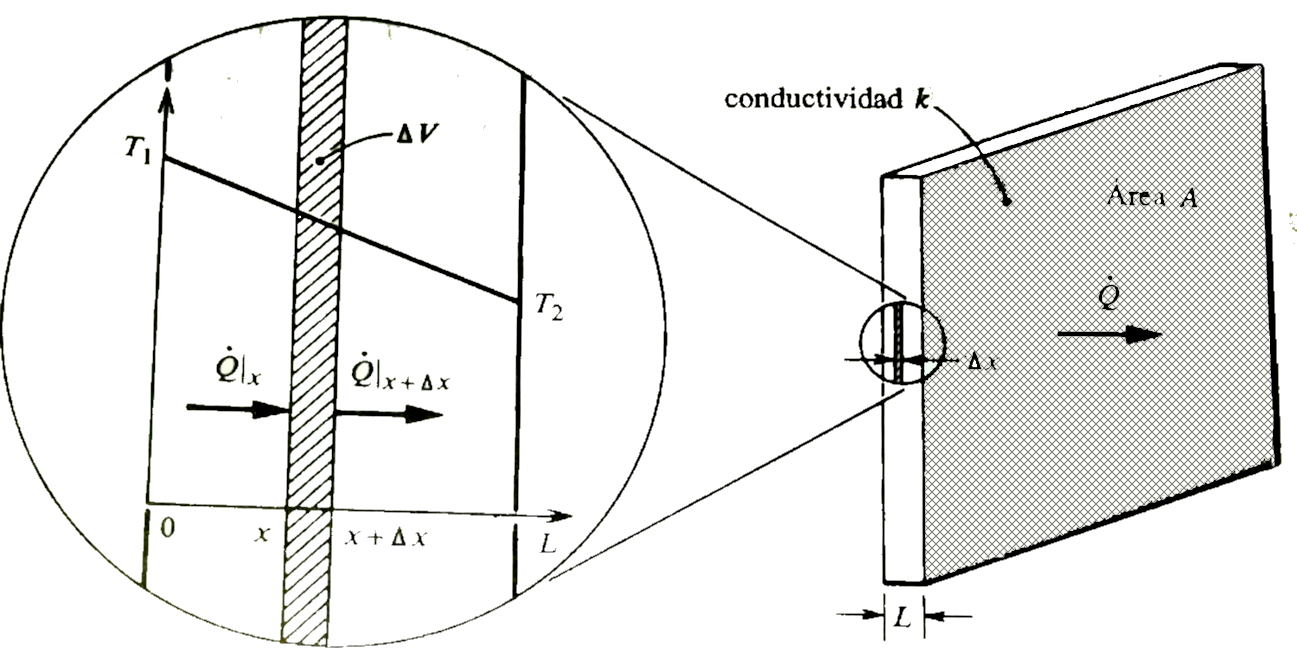
\includegraphics[width=0.6\textwidth]{Imagines/coduccion1pared-nuevo.jpg}
\caption{Conducción unidimencional estacionaria a travez de una pared plana.[Tomado de \cite{Mills} (p.9)]}
\label{fig:cond-paredplana}
\end{figure}

De \ref{eq:leyFourier2} en donde $\dot{Q}$ y $A$ son constantes y que el valor de la conductividad térmica no varie con la temperatura se puede expresar como:



\begin{equation}
    \frac{\dot{Q}}{A}\displaystyle\int_{0}^{L}\, dx = -\displaystyle\int_{T_{1}}^{T_{2}}\,k dT
    \label{eq:intleyFourier1}
\end{equation}

\begin{equation}
    \dot{Q} = \frac{k A}{L} (T_{1}-T_{2})
    \label{eq:intleyFourier2}
\end{equation}




Cabe recalcar que la magnitud de la constante de conductividad térmica, va depender de su estrutura microscopica y de variaciones de la temperatura. De \cite{Warren} se obtuvo la siguiente tabla \ref{Tab:valoresdeconductividad(25C)}  de valores de conductividades térmicas:

\begin{table*} [!ht]
\caption{Valores seleccionados de la conductividad térmica a 300 K (25\textcelsius).[Tomado de \cite{Mills}(p.11)]}

\label{Tab:valoresdeconductividad(25C)}
\begin{center}
\begin{tabular}{| c | c | }
\hline

\cline{1-2}
\textbf{Material}& \textbf{$\frac{W}{mK}$} \\
\hline 

Cobre & 386  \\
\hline
Aluminio & 204   \\
\hline
Bronce ($70\% Cu, 30\% Zn $) & 111  \\
\hline
Acero dulce & 64  \\
\hline
Acero inoxidable,$18-8$ & 15  \\
\hline
Mercurio & 8.4  \\
\hline
Concreto & 1.4  \\
\hline
Vidrio pyrex & 1.09  \\
\hline
Agua & 0.611  \\
\hline
Neopreno & 0.19  \\
\hline
Aceite para motores,$SAE 50$ & 0.145  \\
\hline
Cloruro de polivinilo $(PVC)$ & 0.092  \\
\hline
Freón 12 & 0.071  \\
\hline
Corcho & 0.043  \\
\hline
Fibra de vidrio (densidad media) & 0.038  \\
\hline
Poliestireno & 0.028  \\
\hline
Aire & 0.027  \\
\hline

\end{tabular}
\end{center}
\end{table*}

La ley de Fourier \ref{eq:leyFourier1} se expresa de manera unidimensional para una una mejor compresión pero, se puede representar de forma vectorial, debido a que en la vida real la transferencia de calor puede fluir en cualquier dirección, por ende se puede representar la ley de Fourier de forma más general.

\begin{equation}
\dot{Q} = -k(\frac{\partial T}{\partial x} + \frac{\partial T}{\partial y} + \frac{\partial T}{\partial z})   
    \label{eq:Fouriervectorialmente}
\end{equation}

\begin{equation}
\dot{Q} = -k\nabla T   
    \label{eq:Fouriernabla}
\end{equation}

\cite[p\ 1-2]{Warren} Donde $\nabla$ es el operador tridimencional y $T$ es el campo de temperatura escalar. Se ha visto que el vector flujo de calor $\dot{Q}$ en realidad representa una corriente de calor (energía térmica) que fluye en la dirección del gradiente de temperatura más pronunciado.



\subsubsection{Radiación térmica}

\cite[p\ 13-14]{Mills} Toda la materia y todo el espacio contienen radiación electromagnética. La partícula, o cuanto, de energía electromagnética es el fotón, y la transferencia de calor por radiación puede considerarse tanto en función de ondas electromagnéticas como en función de fotones. El flujo de energía radiante que incide sobre una superficie se conoce como irradiación, $G [\frac{W}{m^2}]$;  el flujo de de energía que abandona una superficie por emisión y reflexión de radiacción electromagnetica se le conoce como $J [\frac{W}{m^2}]$. Una superficie negra (cuerpo negro) se define como aquella que absorbe la totalidad de radiación incidente sin reflejar nada. En consecuencia, toda la radiación que proviene de una superficie negra es emitida por dicha superficie y se expresa mediante la ley de Stefan-Boltzmann:

\begin{equation}
    J = E_{b} = \sigma T^4
     \label{eq:Boltzmann1}
\end{equation}
 
 Donde $E_{b}$ es la potencia del cuerpo negro, $T$ es la temperatura absoluta $[K]$ y $\sigma$ es la constante de Stefan-Boltzmann $(\simeq 5.67x10^{-8})$ $[\frac{W}{m^2 K^4}]$. En el equilibrio, la temperatura del objeto es $T_{2}$, el flujo de radiación que incide sobre el objeto debe de ser igual al flujo de radiación que lo abandona, en donde $ G = \sigma T_{2}^{4}$ como se muestra en la figura \ref{fig:objetonegroconvexo}
 
 \begin{equation}
 G_{1}A_{1} = J_{1}A_{1} = \sigma T_{2}^{4}A_{1} 
     \label{eq:Boltzmann2}
 \end{equation}
 
 Si se aumentará la temperatura, entonces el flujo de calor por radiación a tráves de la superficie, $q_{1}$ es la radiación $[J_{1}]$ menos la irradiación $[G_{1}]$:
 
 \begin{equation}
    q_{1}= J_{1}-G_{1} = \sigma (T_{1}^{4} - T_{2}^{4})
     \label{eq:Boltzmann3} 
 \end{equation}
 
 \begin{figure}[H]
\centering
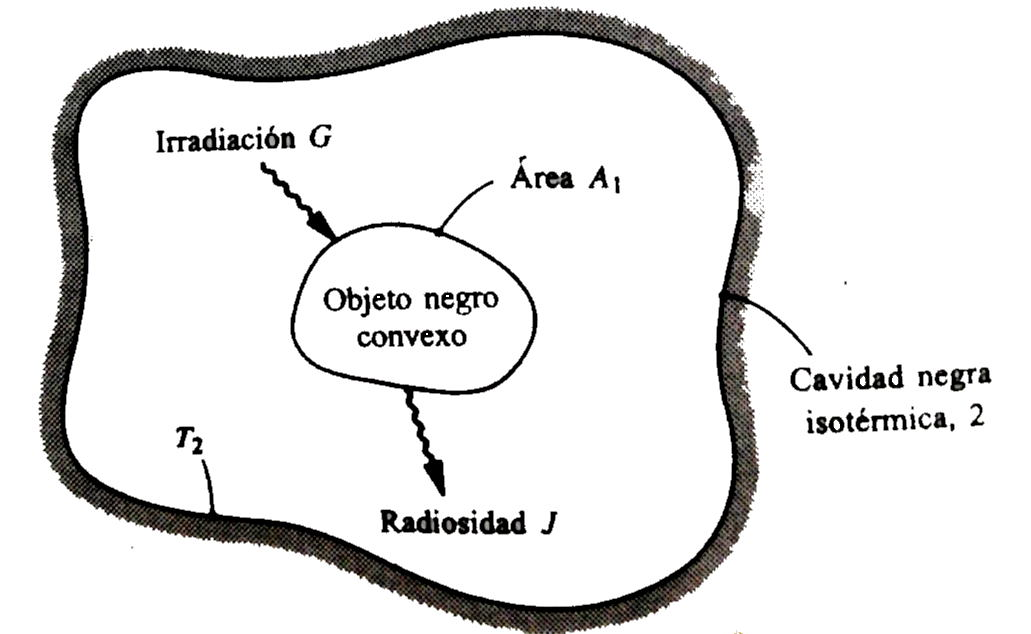
\includegraphics[width=0.6\textwidth]{Imagines/objetonegroconvexo-nuevo.jpg}
\caption{Objeto negro convexo dentro de un recinto (superficie 1) negro isotérmico (superficie 2).[Tomado de \cite{Mills} (p.14)]}
\label{fig:objetonegroconvexo}
\end{figure}
 
 \cite[p\ 15-16]{Mills} El cuerpo negro es una superficie ideal. Las superficies reales absorben menos radiación que las superficies negras. La fracción de la radiación incidente que se absorbe se llama absorbancia (absortividad) $[\alpha]$. Un modelo muy usado para una superficie real es el de la superficie gris, definida para la cual $[\alpha]$ es constante, independientemente de la naturaleza de la radiación incidente. La fracción de la radiación incidente que se refleja es la reflectancia (reflectividad) [$\rho$]. Si el objeto es opaco, es decir, si no es transparente a la radiación electromagnética, entoces $[\rho = 1 - \alpha]$.
 Las superficies reales también emiten menos radiación que las superficies negras. La fracción emitida de la potencia de emisión de cuerpo negro $\sigma T^{4}$ se conoce como emitancia (emisividad $[\epsilon]$). En una superficie gris el valor de la emitancia y la absorbancia son iguales $[\epsilon = \alpha]$.
 Si se transfiere calor entre dos superficies grises finitas, como muestra la figura  [\ref{fig:transradiacion}] la velocidad de flujo de calor dependerá de las temperaturas $T_{1}$ y $T_{2}$ y de las emitancias $\epsilon_{1}$ y $\epsilon_{2}$, asi como de la geometría.
 
\begin{equation}
\dot Q_{12}= A_{1}F_{12} (\sigma T_{1}^{4}-\sigma T_{2}^{4})
    \label{eq:Radiacion}
\end{equation}

\begin{figure}[H]
\centering
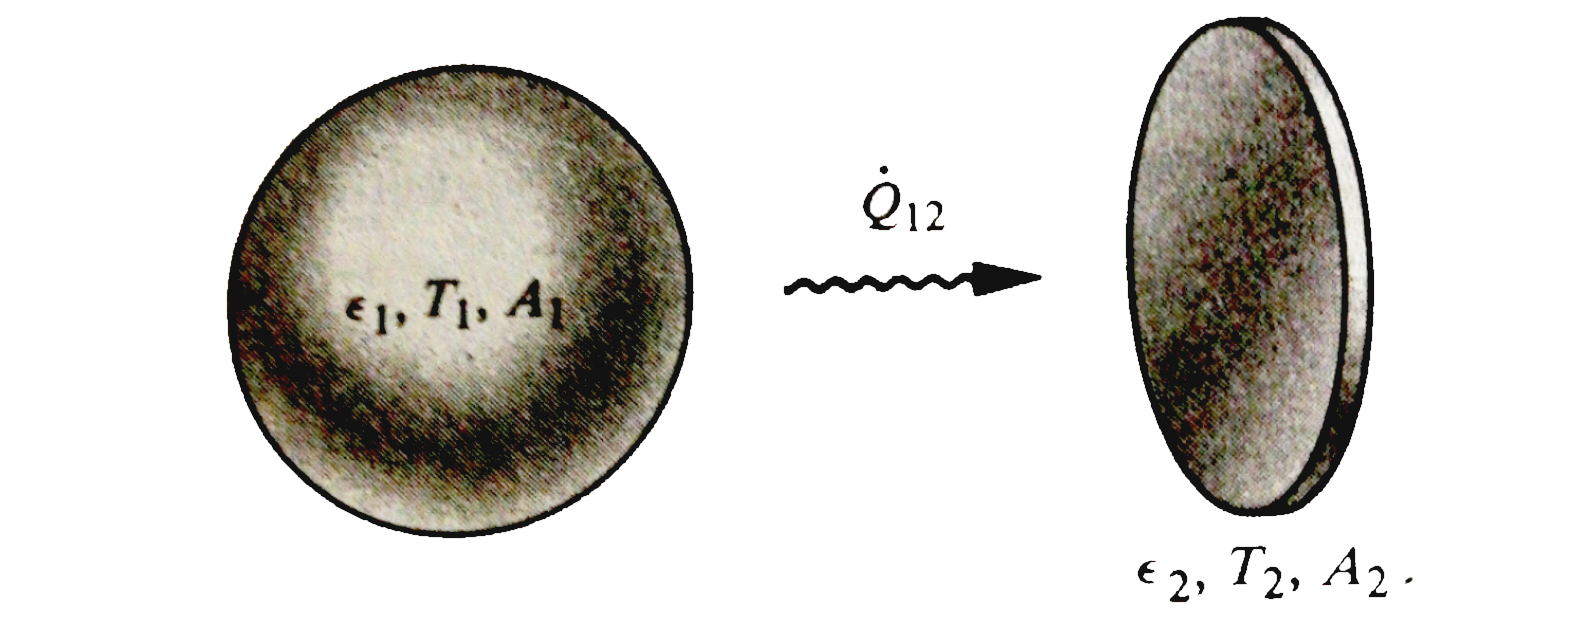
\includegraphics[width=0.6\textwidth]{Imagines/transradiacion-nuevo.jpg}
\caption{Transferencia de calor por radiación entre dos superficies grises finitas.[Tomado de \cite{Mills} (p.16)]}
\label{fig:transradiacion}
\end{figure}


En donde $\dot{Q_{12}}$ es el intercambio neto de energía radiante de la superficie $1$ a la superficie $2$ y $F_{12}$ es el factor de transferencia el cual depende de las emitancias y la geometria. En la figura [\ref{fig:transradiacion}] se puede decir que $F_{12} \simeq \epsilon_{1}$ asumiendo que $A_{2} >> A_{1}$, por lo que la ecuación [\ref{eq:Radiacion}] se convierte en:

\begin{equation}
\dot Q_{12} = \epsilon_{1} A_{1}(\sigma T_{1}^{4}-\sigma T_{2}^{4})
    \label{eq:Radiacion2}
\end{equation}

Debido a que trabajar con un exponente de grado $4$ en $T^{4}$ se hace algo complicado de manejar por tal motivo se descompone:

\begin{equation*}
\dot Q_{12} = \epsilon_{1} A_{1}\sigma (T_{1}^{2} + T_{2}^{2})(T_{1} + T_{2})(T_{1} - T_{2})
    \label{eq:Radiacion3}
\end{equation*}

\begin{equation*}
\simeq  \epsilon_{1} A_{1}\sigma(4T_{m}^{3})(T_{1} - T_{2})
    \label{eq:Radiacion4}
\end{equation*}

En donde $h_{r} = \sigma 4T_{m}^{3} $ es el coeficiente de transferencia de calor por radiación $[\frac{W}{m^2K}]$, la ecuación \ref{eq:Radiacion4} queda de la siguiente manera:

\begin{equation}
\dot Q_{12} = A_{1} h_{r} (T_{1} - T_{2})
    \label{eq:Radiacion5}
\end{equation}

 
 
 
 




\subsubsection{Convección de calor}
\cite[p\ 18]{Mills} La convección de calor es un término que se usa para describir la transferencia de calor de una superficie a un fluido en movimiento. La superficie puede ser el interior de una tubería el fuselaje de avión supersóníco o la interfaz entre el agua y el aire de una torre de enfriamiento. El flujo puede ser forzado, como en el caso de un líquido que se bombea a través de una tubería o del aire sobre un avión que surca la atmósfera. por otro lado el flujo podría se natural, causado por fuerzas de empuje 
debidas a una diferencia de densidad, como en el caso de una torre de enfriamiento de corriente natural.
Estos dos tipos de flujo pueden ser internos, como en el de la tubería, o externos, como el flujo sobre el avión. Además, un flujo ya sea forzado o natural, puede ser laminar o turbulento, el flujo laminar es más común cuando las velocidades son bajas, las dimensiones son más pequeñas y los fluidos son más viscosos. El flujo de una tubería llega a ser turbulento cuando el grupo adimensional llamado número de Reynolds $Re_{D} = \frac{VD}{v}$ es mayor que 2300, donde $V$ es la velocidad $[\frac{m}{s^2}]$, $D$ es el diámetro de la tubería $m$ y $v$ es la viscosidad cinemática del fluido $[\frac{m^2}{s}]$. Las velocidades de transferencia de calor tienden a ser mucho mayores en los flujos turbulentos que en los laminares, debido a la mezcla violenta que sufre el fluido.

Al igual, que la conducción de calor la convección de calor posee una constante de proporcionalidad llamada coeficiente de transferencia de calor por convección $h_{c}$ $[\frac{W}{m^2K}]$ en donde, el valor de este coeficiente no es constante el cual varía en rangos según el tipo de fluido, algunas propiedades del mismo como la viscosidad entre otras además, de la velocidad del mismo. Por ende, aunque en la actualidad se tiene valores de coeficientes de tranferencia de calor por convección para ciertos fluidos como se muestra la tabla \ref{Tab:valoresde hc}.

\begin{table*} [!ht]
\caption{Ordenes de magnitud de algunos coeficientes de transferencia de calor medio .[Tomado de \cite{Mills}(p.23)]}

\label{Tab:valoresde hc}
\begin{center}
\begin{tabular}{| c | c | }
\hline

\cline{1-2}
\textbf{Flujo y fluido} & \textbf{$\frac{W}{m^2K}$} \\
\hline 

Convección libre, aire & 3-25  \\
\hline
Convección libre, agua & 15-100   \\
\hline
Convección forzada, aire & 10-200  \\
\hline
Convección forzada,agua & 50-10000  \\
\hline
Convección forzada, sodio líquido & 10000-100000  \\
\hline
Condesación de vapor & 5000-50000  \\
\hline
Ebullición de agua & 3000-100000  \\
\hline
\end{tabular}
\end{center}
\end{table*}

La ecuación que describe la convección de calor se suele llamar ley de enfriamiento de Newton, aunque más bien se trata de una definición de $h_{c}$ y no de la verdadera ley física. En donde, el flujo de calor de la superficie del fluido  $q_{s}$ [$\frac{W}{m^2}$], la temperatura de la superfcie $T_{s}$ y la temperatura del entorno $T_{e}$.

\begin{equation}
    q_{s} = \frac{\dot{Q}}{A} = h_{c}\Delta T = h_{c}(T_{s}-T_{e})
    \label{eq:ecuaciondeconvección}
\end{equation}

El problema radica en que el $h_{c}$ va variar según el tipo de fluido ya sea laminar o tubulento asimismo, de la geometria por donde se mueve el fluido. Por ende, sea han desarrollado mecanismo para obterner el coeficiente de convección de calor como lo es número de Reynolds el cual determina si un fluido es laminar o turbulento o se encuentra en medio de los dos, en el que él mismo puede variar según la geometría y si es de forma forzada o natural. Según el autor Yunus \cite[p\ 540]{yunus}. La transición de fluido laminar a turbulento depende de la geometría, rugosidad de la superficies, velocidad del fluido, temperatura de la superficie y del tipo de fluido entre otras cosas.
El regimen del fluido depende principalmente del radio de fuerza inercial o fuerza de viscosidad de el fluido. En donde   velocidad de fluido $V_{avg}$ $[\frac{m}{s}]$, diametro para este caso pero va a depender de la geometría o también se le llama diametro hidráulico $D_{h}$ $\frac{4A_{c}}{perímetro}$ lo cual se puede observar en la figura \ref{fig:diametrohidraulco} $ D $ $[m]$, viscosidad cinemática de el fluido $v =\frac{\mu}{\rho}$ $[\frac{m^2}{s}]$

\begin{figure}[H]
\centering
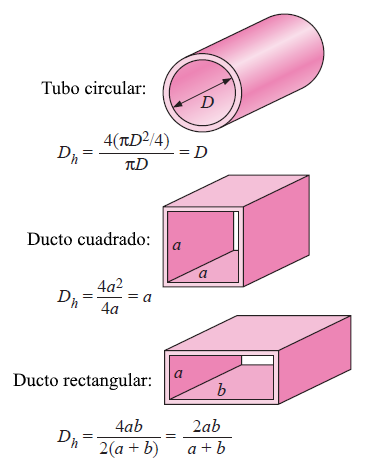
\includegraphics[width=0.4\textwidth]{diametrohidraulico-nuevo.png}
\caption{Diametros hidraulicos.[Tomado de \cite{yunus} (p.540)]}
\label{fig:diametrohidraulco}
\end{figure}

\begin{equation}
Re = \frac{F. inercial}{F. viscosa} = \frac{V_{avg}D}{v} = \frac{\rho V_{avg}D}{\mu}
    \label{eq:reynolds}
\end{equation}

En el caso de tubos circulares el número de Reynolds determina si el fluido es laminar, turbulento o si se encuentra en medio de ambos. Por eso los rangos en que se clasifican lo ya antes mencionados estan:


\begin{enumerate}
    \item Fluido laminar: Re < 2300
    \item Fluido trancitorio: 2300 <= Re <= 4000
    \item Fluido turbulento: Re > 4000
\end{enumerate}

Cuando se esta en el caso de convección forzada una manera de poder encontrar el coefciente de transferencia de calor por convección es mediante número de Nusselt, este fue gracias a Wilhelm Nusselt. Pero, es de recalcar que el número de Nusselts cambia según su geometría, temperatura entre otras variables más, esta ecuación relaciona la constante de conductividad térmca con el coeficiente de transferencia de calor por convección:

\begin{equation}
Nu = \frac{h_{c}L}{k}
    \label{eq:Nusselt}
\end{equation}

Cabe recalcar que el número de Nusselt depende de variables como el número de Reynolds y número de Prandtl $F_{Nu} = (Re,Pr)$ este último fue por el aporte de Ludwig Prandtl, el cual realizó contribuciones a la teoría de capa límite. En el caso, del número de Nusselt se presentará en casos como en placas planas, cilindros, flujo uniforme. \cite[p\ 812-813]{yunus} 

\begin{enumerate}
    \item Placas planas: 
    
\begin{equation}
 Re < 5x10^{5} = Laminar: Nu = 0.664Re^{0.5}Pr^{1/3}
    \label{eq:p.planaslaminar}
\end{equation}

\begin{equation}
 \frac{0.6 \leq Pr \leq 60}{5x10^{5} \leq Re \leq 10^{7}} = Turbulento: 0.037Re^{0.8}Pr^{1/3}
 \label{eq:p.planasturbulento}
\end{equation}

\begin{equation}
\frac{0.6 \leq Pr \leq 60}{5x10^{5} \leq Re \leq 10^{7}} = Turbulento: (0.037Re - 871)^{0.8}Pr^{1/3}
    \label{eq:p.planascombinado}
\end{equation}

\item Cilindro:

\begin{equation}
Re Pr > 0.2 = Nu = 0.3 + \frac{0.62Re^{1/2}Pr^{1/3}}{[1 + (0.4/Pr)^{2/3}]^{1/4}}[1 + (\frac{Re}{282000})^{5/8}]^{4/5}
    \label{eq:p.cilindro}
\end{equation}

\item Flujo de calor uniforme:

\begin{equation}
Laminar: Nu_{x} = 0.453Re_{x}^{0.5}Pr^{1/3}
    \label{eq:p.flujoconst.laminar}
\end{equation}

\begin{equation}
Turbulento: Nu_{x} = 0.453Re_{x}^{0.8}Pr^{1/3}
    \label{eq:p.flujoconst.turbulento}
\end{equation}
\end{enumerate}

\subsection{Propiedades elementales de un sistema hidráulico}

Un sistema  hidráulico tiene cinco parámetros de importancia: la presión, la masa del flujo, temperatura, densidad y volumen del flujo.
Para fluidos incompresibles (volumen se mantiene constante), según la ley de conservación de la masa tiene que:

\begin{equation}
m=\int \rho fdt     
\label{eq:flujo}
\end{equation}

donde en \ref{eq:flujo}, m es el flujo neto de la masa, $\rho$ es la densidad del fluido, además $dV/dt = f = f_i - f_o$ es el volumen neto del flujo, por lo tanto:

\begin{equation}
\frac{dm}{dt} = \rho \frac{dV}{dt} = \rho f     
\label{eq:flujo}
\end{equation}

\newpage
\section{Modelo matemático de un proceso que incluye un serpentín con intercambiador }

\subsection{Descripción de funcionamiento}

El modelo matemático siguiente se basa en un proceso típico del calentamiento de un líquido que fluye a través de un intercambiador de calor, mnediante un vapor que se mueve por un serpentín instalado en su interior. En el modelado del serpentín además se deberá considerar el efecto de la consdensación del vapor que circula por este por medio de una constante de nivel de humedad (\lambda).



\subsection{Suposiciones importantes para el modelado}

\begin{itemize}
    
\item Se supone un fluido incompresible, por lo que el volumen del líquido se mantiene constante.

\item Se supone un flujo laminar para el líquido transportado en el serpentín.

\item Se desprecian las pérdidas de calor a través del tanque.
\end{itemize}


\subsection{Asignación}

Las variables de estado están dadas por:

\begin{itemize}

\item $T(t)$: Temperatura en el tanque intercambiador
\item $T_s(t)$: Temperatura del serpentín
\end{itemize}

Con las entradas:
\begin{itemize}
\item $T_i(t)$: Temperatura de flujo de entrada en tanque intercambiador
\item $w(t)$ Caudal del vapor que pasa por el serpentín
\end{itemize}

\subsection{Balance de energía}
El dispositivo requiere que el diferencial de volumen sea constante por lo que el volumen que entra sea igual al de entrada.
\begin{equation}
\rho \frac{\mathrm{d} V }{\mathrm{d} t} = f_1 (t) \rho  - f_2 (t) \rho
\label{eq:volumen}
\end{equation}

Para un correcto funcionamiento del intercambiador es necesario que los flujos de entrada y salida sean iguales y constantes.
\begin{equation}
    f_1(t) = f_2(t) = f(t)
    \label{eq:Flujos}
\end{equation}

Por lo tanto el volumen será constante.

\subsection{Balance de energía en el intercambiador}
Para mantener el balance del fluido contenido en el intercambiador se determina la siguiente ecuación: \\
 \begin{equation}
V \rho C_{V}\frac{\mathrm{d} T(t)}{\mathrm{d} t}= f(t)\rho C_{p}T_{i}(t) +UA[T_{s}(t)-T(t)]-f(t)\rho C_{p}T(t)
\label{eq:BalanFlui}
 \end{equation}
Con $V$ Volumen del intercambiador en $m^3$, $\rho$ la densidad del líquido en el intercambiador en $kg/ m^3$, A el área de transferencia de calor en $m^2$ y $T_s(s)$ la temperatura del líquido primario del serpentín en $^{\circ}$K.

\subsection{Balance de energía en el serpentín}
A través del serpentín, que está sumergido y que transporta el líquido que introduce el calor al sistema debe conservar balance de energía según la ecuación: \\
\begin{equation}
C_{M}\frac{\mathrm{d} T_{s}(t)}{\mathrm{d} t} = w(t)\lambda - UA[T_s (t)- T(t)]
\label{eq:EnergSerp}
\end{equation}

con w(t) del flujo de vapor en $kg/s$ y $C_M$ es la capacidad calórica del metal del serpentín en $J/^{\circ}$K; además debe cumplirse que el $C_V$ del líquido contenido en el intercambiador y el $C_p$ de la masa que que se quiere calentar sean aproximadamente iguales. También que la temperatura de la corriente de alimentación del fluido primario se mantenga constante.
Además, las incognitas del modelo son cuatro:
\begin{itemize}
    \item T    temperatura del líquido en el intercambiador.
    \item $T_s$   temperatura del líquido en serpentín.
    \item $\lambda$   flujo de corriente del líquido.
    \item w    flujo de vapor
\end{itemize} 


\subsection{Transformada de Laplace}
Con el fin de analizar la respuesta controlada del proceso se requiere linealizar las ecuaciones del modelo, en función del tiempo.
De ahí que se obtiene el balance de energía linealizado a través del intercambiador a partir de la ecuación \ref{eq:BalanFlui}.

\begin{equation}
V_{\rho \;} C_V \frac{dT \left(t\right)\;}{\;d\left(t\right)}=\rho \;C_{P\;} \left(T_i(t) -T(t) \right)f\left(t\right)+\mathrm{UA}T  _S \left(t\right)-\left(\mathrm{UA}+f(t) \rho \;C_P \right)T \left(t\right)
\end{equation}

También expresada como en \ref{eq:uno}:

\begin{equation}
    \tau \;\frac{dT\left(t\right)}{\;d\left(t\right)}+T\left(t\right)=K_F f\left(t\right)+K_s T_s \left(t\right)
    \label{eq:uno}
\end{equation}


donde:

\begin{equation}
    \tau =\frac{V_{\rho \;} C_p }{{\;\mathrm{UA}+f(t) \rho } {C_P }}\;
\end{equation}

\begin{equation}
 K_F =\frac{\rho \;C_p \left(T_i (t) -T(t) \right)}{\mathrm{UA}+f(t) \rho C_P } 
\end{equation}

\begin{equation}
K_s =\frac{\mathrm{UA}}{\mathrm{UA}+f(t) \rho C_P  } 
\end{equation}

Se tiene también el balance de energía a través del serpentín linealizado:

\begin{equation}
C_M \frac{dT  _S \left(t\right)}{\;d\left(t\right)}=w\left(t\right)\lambda -\mathrm{UA}T  _S\left(t\right)+\mathrm{UA}T \left(t\right)
\label{eq:dos}
\end{equation}

También expresada como:

\begin{equation}
\tau  _C \frac{dT  _S \left(t\right)}{\;d\left(t\right)}+T  _S \left(t\right)=T \left(t\right)+K_w
\end{equation}

Con:

\begin{equation}
\tau  _C =\frac{C_M }{\mathrm{UA}}
\end{equation}

\begin{equation}
K_W =\frac{\lambda }{\mathrm{UA}}\;
\end{equation}

Las funciones de transferencias relevantes para este sistema se obtienen al aplicar la transformada de Laplace para las ecuaciones \ref{eq:uno} y \ref{eq:dos}.

Para el líquido a través del intercambiador la ecuación \ref{eq:tres}.

\begin{equation}
T \left(s\right)=\frac{K_F }{\tau s+1}F\left(s\right)+\frac{K_S }{\tau s+1}T_s \left(s\right)
\label{eq:tres}
\end{equation}

Mientras que para el vapor a través del serpentín la ecuación \ref{eq:cuatro}.


\begin{equation}
T_s \left(s\right)=\frac{1}{\tau  _C s+1}T \left(s\right)+\frac{K_W }{\tau_C s+1}W\left(s\right)
\label{eq:cuatro}
\end{equation}

A partir de las dos funciones transferencia anteriores se puede asegurar que el modelo cuenta con dos variables de estado, con dos variables de entrada. Sustituyendo la ecuación \ref{eq:cuatro} en la ecuación \ref{eq:tres}, se obtiene la función de transferencia de la temperatura en el intercambiador con respecto a las variables de entrada:



\begin{equation}
T \left(s\right)=\frac{K_W K_S }{\left(\tau  _C s+1\right)\left(\tau s+1\right)-K_{S\;} }W\left(s\right)+\frac{K_F \left(\tau  _C s+1\right)}{\left(\tau  _C s+1\right)\left(\tau s+1\right)-K_{S\;} }F\left(s\right)
\end{equation}

En donde:

\begin{equation}
G_W \left(s\right)=\frac{K_W K_S }{\left(\tau_C s+1\right)\left(\tau s+1\right)-K_S }
\end{equation}

\begin{equation}
G_F \left(s\right)=\frac{K_F \left(\tau  _C s+1\right)}{\left(\tau  _C s+1\right)\left(\tau s+1\right)-K_S }
\end{equation}

%\subsection{Dinámica de la válvula de control}

%Para una válvula de igual porcentaje con caída de presión constante se tiene la función de transferencia en \ref{eq:cinco}.

%\begin{equation}
%G_V \left(s\right)=\frac{W\left(s\right)}{M\left(s\right)}=\frac{K_V }{\tau  _V s+1}
%\label{eq:cinco}
%\end{equation}

%Con $K_V$ la ganancia de la válvula calculada de la siguiente forma:

%\begin{equation}
%K_V =\frac{\bar{w} \mathrm{ln}\left(a\right)}{100}
%\end{equation}

%\subsection{Dinámica del sensor transmisor}

%\begin{equation}
%%H\left(s\right)=\frac{C\left(s\right)}{T\left(s\right)}=\frac{K_T }{\tau  _T s+1}
%\end{equation}

%\begin{equation}
%K_T =\frac{100-0}{200-100}=1\ldotp 0\frac{TO}{^{\circ} F\;}
%\end{equation}

\subsection{Parámetros a utilizar en simulación}

\begin{itemize}
   
 \item $A=241.5 \; pie^2$

 \item $C_m = 265.7 \; BTU/ ^{\circ}F$

%\item $\tau _T = 0.75 \; min$

\item $\tau _C = 0.524 \; min$

\item $K_W = 1.905 \; ^{\circ}F/(lb/min)$

%\item $K_SP = K_T = 1.905 ^{\circ}F/(lb/min)$

\item $V = 120 \; pie^3$

\item $\tau _V = 0.20 \; min$

\item $K_F = -2.06  \; ^{\circ}F/(pie^3 /min)$

\item $K_S = 0.383 \; ^{\circ}F/^{\circ}F$

Parámetros tomados de \cite{Natividad}, que toman como referencia los patrones de mediciones más usuales en la industria. Esto considerando que se pueden utilizar diferentes tipos de aceites y líquidos térmicos.
\end{itemize}

\newpage

Para la elaboración de la tabla [\ref{Tab:dimencionesserpentin}] se empleo los anexos de dimenciones de tubos de aceros al carbono obtenido de  \cite{vemacero}. Además, se utilizó las dimenciones propuestas en \cite{Burbano} [Ver Anexo] asimismo, para el cálculo del el aréa del serpentín se usó la ecuación $A_{s} = \frac{\pi D^2_{nom}}{4}$ y el volumen $V_{s} = A_{s}L_{s}$.

\begin{table*} [!ht]
\caption{Dimensiones del serpentín de un tubo de acero al carbono(AISI 1010)[Elaboración propia]}

\label{Tab:dimencionesserpentin}
\begin{center}
\begin{tabular}{| c | c | }
\hline

\cline{1-2}
\textbf{Dimensiones}& \textbf{Valores} \\
\hline 

Diametro Nominal \ [$mm$] & 15  \\
\hline
Espesor \ [$mm$] & 2.77   \\
\hline
Longitud Total \ [$mm$] & 1644 \\
\hline
Area \ [$m^2$]  & 0.00017671   \\
\hline
Volumen \ [$m^3$] & 0.00029052   \\
\hline
\end{tabular}
\end{center}
\end{table*}


\begin{itemize}
    \item $A_{s}$ = Aréa del serpentín. 
    \item $E_{s}$ = Espesor del sepertín.
    \item $L_{s}$ = Longitud total del serpentín.
    \item $D_{s}$ = Diametro nominal del serpentín.
    \item $V_{s}$ = Volumen del serpentín.
\end{itemize}



\begin{table*} [!ht]
\caption{Dimensiones de la carcasa de un tubo de acero inoxidable (AISI 302)[Elaboración propia]}

\label{Tab:dimencioncarcas}
\begin{center}
\begin{tabular}{| c | c | }
\hline

\cline{1-2}
\textbf{Dimensiones}& \textbf{Valores} \\
\hline 

Diametro Nominal \ [$mm$] & 187  \\
\hline
Espesor \ [$mm$] & 13   \\
\hline
Longitud Total \ [$mm$] & 670 \\
\hline
Area \ [$m^2$]  & 0.027465   \\
\hline
Volumen \ [$m^3$] & 0.018401   \\
\hline
Diámetro de entrada $F$ [$mm$] & 26 \\
\hline
\end{tabular}
\end{center}
\end{table*}

Los valores de los parámetros empleados para el dimencionado de la carcasa son los siguientes:

\begin{itemize}
    \item $D_{c}$ = Diámetro nominal de la carcasa.
    \item $E_{c}$ = Espesor de la carcasa.
    \item $L_{c}$ = Longitud total de la carcasa.
    \item $A_{c}$ = Área de la carcasa.
    \item $V_{c}$ = Volumen de la carcasa.
    \item $Di_{c}$ = Diamentro de entrada del fluido.
\end{itemize}




En la tabla [\ref{tab:flujodemasa}] los datos empleados son a $1 \ atm$, estos valores se tomarón de las referencias \cite{yunus} \cite{Warren} [ver Anexos]. Este es un ejemplo de los valores de los parámetros para el cálculo de los flujos de masa tanto del agua como del serpentín, los cuales varían según la temperatura del fluido, asimismo los valores de los caudales pueden variar.

\begin{table*}[!ht]
\caption{Flujos de calor de masas del agua y el aire a $1 atm$  [Elaboración propia]}
\centering
\begin{tabular}{|c|c|c|c|c|}
\hline
& \multicolumn{4}{c|}{Calor por flujo de masa} \\
\cline{2-5}
& Temperatura$[^{\circ}C]$ & Densidad$[\frac{Kg}{m^3}]$ & Capacidad calorifica$[\frac{J}{KgK}]$ & Caudal$[\frac{m^3}{s}]$ \\
\hline \hline
\multirow{1}{1cm}{Agua} & 10 $\approx$ 283.15 K & 999.77 & 4.193 & 0.5\\ \cline{1-5}
\cline{1-4}
Aire & 40 $\approx$ 313.15 K & 1.127 & 1007 & 2 \\ \cline{1-5}
\end{tabular}
\label{tab:flujodemasa}
\end{table*}

\begin{itemize}
    \item $Ti_{h}$ = Temperatura inicial del agua.
    \item $\rho i_{h}$ = Densidad inicial del agua.
    \item $Cpi_{h}$ = Capacidad calorifica del agua.
    \item $Ti_{a}$ = Temperatura inicial del aire.
    \item $\rho i_{a}$ = Densidad inicial del aire.
    \item $Cp i_{a}$ = Capacidad calorifica del aire.
\end{itemize}

Las resistencias térmicas de la carcasa de acero inoxidable (AISI 302) y el serpentín de acero al carbono (AISI 1010), se calcularon mediante la ecuación [\ref{eq:resistencia termica}] además, para los valores de conductividades térmicas se emplearon los que se cuentran en Anexos. La resistencia térmica esta dada en $[\frac{^{\circ}C s}{J}]$ y la conductividad térmica en $[\frac{W}{m ^{\circ}C}]$, cuyos valores varían según la temperatura la cual esta dada en Kelvin.

Suponiendo que la temperatura máxima del serpentín (AISI 1010) y  es de $400K$ Su conductividad térmica es de $58.7$ [\ref{fig:propiedadesmetales1}] y de igual forma,la temperatura máxima de la carcasa (AISI 302) es de $400 K$ cuya conductividad térmica es de $17.3$ [\ref{fig:propiedadesmetales2}].

\begin{itemize}
    \item $R_{TSc}$ = Resistencia térmica del serpetín-carcasa $[\frac{^{\circ}C s}{J}]$.
     \item $R_{TCa}$ = Resistencia térmica de la carcasa-ambiente $[\frac{^{\circ}C s}{J}]$.
     \item $\sigma_{s}$ = Conductividad térmica de la serpentín $[\frac{W}{m ^{\circ}C}]$.
     \item $\sigma_{c}$ = Conductividad térmica de la carcasa $[\frac{W}{m ^{\circ}C}]$.
\end{itemize}

\begin{equation}
R_{T} = \frac{L}{\sigma A} \ [\frac{^{\circ}C s}{J}] \label{eq:resistencia termica}\\ 
\end{equation} 

\begin{equation}
R_{TSc} = \frac{L_{s}}{\sigma_{Sc} A_{s}} = 158.49[\frac{^{\circ}C s}{J}]   \label{eq:resistencia termica serpentin}\\
\end{equation} 

\begin{equation}
R_{TCa} = \frac{L_{c}}{\sigma_{Ca} A_{c}} = 1.410[\frac{^{\circ}C s}{J}] \label{eq:resistencia termica carcasa}
\end{equation} 

De la ecuación [\ref{eq:captermserpentin}][\ref{eq:resistencia termica carcasa}] se puede obtener la capacidad térmica tanto del cerpetín (AISI 1010) como el de la carcasa (AISI 302). Tomando en cuenta que el área del serpetín es el espesor del tubo y no el área total por lo que se obtiene $As_{e} = \frac{\pi (2.77mm)^{2}}{4} = 6.026 \ 10^{-6}m^{2}$ y de igual forma el área de la carcasa $Ac_{e} = \frac{\pi (13mm)^{2}}{4} = 132.733 \ 10^{-6}m^{2}$. De [\ref{fig:propiedadesmetales1}] se obtiene una densidad y capacidad calorífica del serpentín respectivamente de $7832 $ y $559$ y de [\ref{fig:propiedadesmetales2}] se obtiene una densidad y capacidad calorífica respectivamente para la carcasa de $8055$ y $512$ ambos con su temperatura máxima de $400K$. Por lo que evaluando los valores se obtiene: 

\begin{align} 
Ct_{s} = M_{s}Cp_{s} = Cp_{s} \rho_{s}V_{s} = Cp_{s} \rho_{s}A_{s}L_{s} = 43.373[\frac{J}{K}] \label{eq:captermserpentin}\\ 
Ct_{c} = M_{c}Cp_{c} = Cp_{c} \rho_{c}V_{c} = Cp_{c} \rho_{c}A_{c}L_{c} = 366.766 [\frac{J}{K}] \label{eq:capatermicarcasa}
\end{align}

Donde:

\begin{itemize}
    \item $Ct_{s}$ = Capacidad térmica del serpentín $[\frac{J}{K}]$ 
    \item $M_{s}$ = Masa del serpentín $[Kg]$
    \item $Cp_{s}$ = capacidad calorífica del  serpentín $[\frac{J}{Kg\ K}]$
    \item $Ct_{c}$ = Capacidad térmica del carcasa $[\frac{J}{K}]$
    \item $M_{c}$ = Masa del carcasa $[Kg]$
    \item $Cp_{c}$ = capacidad calorífica del carcasa $[\frac{J}{Kg\ K}]$
    
\end{itemize}

De igual manera, para obtener los resistores térmicos el primero del serpentín a la carcasa y el otro de la carcasa al ambiente ambos mediante un flujo de calor. Sustituyendo los valores de [\ref{eq:resistencia termica serpentin}][\ref{eq:resistencia termica carcasa}] en [\ref{eq:resistor ser-car}][\ref{eq:resistor car-amb}]

\begin{itemize}
    \item $W_{sc}$ = Flujo de calor del serpentín a la carcasa $[\frac{J}{s}]$.
    \item $W_{ca}$ = Flujo de calor de la carcasa al ambiente $[\frac{J}{s}]$.
    \item $T_{s}$ = Temperatura del serpentín $[K]$.
    \item $T_{c}$ =Temperatura del carcasa $[K]$.
    \item $T_{amb}$ =Temperatura del ambiente $[K]$.
\end{itemize}

\begin{equation}
W_{sc} = \frac{T_{s} - T_{c}}{R_{TSc}} = \frac{T_{s} - T_{c}}{158.49} \label{eq:resistor ser-car}\\ 
\end{equation} 


\begin{equation}
W_{ca} = \frac{T_{c} - T_{amb}}{R_{TCa}} = \frac{T_{c} - T_{amb}}{1.410} \label{eq:resistor car-amb}
\end{equation} 

La figura [\ref{fig:DCLtermico}] de abajo presenta el diagrama de cuerpo libre térmico.


\begin{figure}[H]
\centering
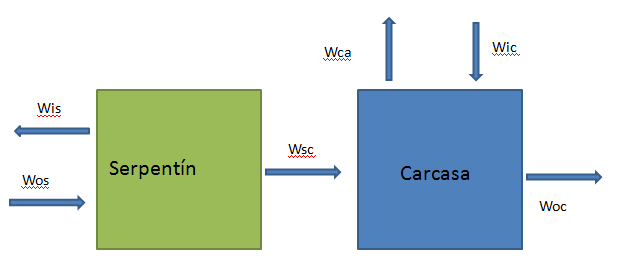
\includegraphics[width=0.8\textwidth]{Imagines/DCLtermico.png}
\caption{Diagrama de cuerpo libre térmico.}
\label{fig:DCLtermico}
\end{figure}

\begin{itemize}
    \item $W_{is}$ = calor por un flujo de masa entrando al serpentín. 
    \item $W_{os}$ = calor por un flujo de masa saliendo del serpentín.
    \item $W_{sc}$ = calor por un flujo de masa serpentín-carcasa.
    \item $W_{ca}$ = calor por un flujo de masa carcasa-ambiente.
    \item $W_{ic}$ = calor por un flujo de masa entrando a la carcasa.
    \item $W_{oc}$ = calor por un flujo de masa saliendo de la  carcasa.
\end{itemize}

Ley de calor de fourier para el serpentín:

\begin{equation} 
Ct_{s} \dot T_{s} = W_{is} - W_{os} - W_{sc}\\
\end{equation} 

\begin{equation} 
Ct_{s} \dot T_{s} = \rho_{is}Q_{is}Cp_{is}T_{is} - \rho_{os}Q_{os}Cp_{os}T_{os} - \frac{T_{s}-T_{c}}{R_{TSc}}
\end{equation} 

Si las densidades de entrada y salida son iguales $\rho_{is} = \rho_{os} = \rho$, los caudales son iguales $Q_{is} = Q_{os} = Q $ y sus capacidades calorífica de igual forma $Cp_{is} = Cp_{os} = Cp$ asimismo, $T_{os} = T_{s}$:

\begin{equation*}
Ct_{s} \dot T_{s} = \rho Q Cp T{is} - \rho Q Cp T_{s} - \frac{T_{s}-T_{c}}{R_{TSc}}\\
\end{equation*} 

\begin{equation*}
Ct_{s} \dot T_{s} = \rho Q Cp T{is} - T_{s} [\rho Q Cp + \frac{1}{R_{TSc}}] + \frac{T_{c}}{R_{TSc}}
\end{equation*} 

\begin{equation}
\dot T_{s} = \frac{\rho Q Cp}{Ct_{s}} T{is} - T_{s} \frac{1}{Ct_{s}} [\rho Q Cp + \frac{1}{R_{TSc}}] + \frac{1}{Ct_{s}R_{TSc}}T_{c}
     \label{eq:eqdifftempserpentin}
\end{equation}

Ley de calor de Fourier para la carcasa:

\begin{equation*} 
Ct_{c} \dot T_{c} = W_{sc} + W_{ic} - W_{oc} - W_{ca}
\end{equation*}

\begin{equation*} 
Ct_{c} \dot T_{c} = \frac{T_{s} - T_{c}}{R_{TSc}} + \rho_{ic}Q_{ic}Cp_{ic}T_{ic} - \rho_{oc}Q_{oc}Cp_{oc}T_{oc} - \frac{T_{c} - T_{amb}}{R_{TCa}}
\end{equation*}

Si las densidades de entrada y salida son iguales $\rho_{ic} = \rho_{oc} = \rho$, los caudales son iguales $Q_{ic} = Q_{oc} = Q $ y sus capacidades calorífica de igual forma $Cp_{ic} = Cp_{oc} = Cp$ asimismo, $T_{oc} = T_{c}$:

\begin{equation*} 
Ct_{c} \dot T_{c} = \frac{T_{s} - T_{c}}{R_{TSc}} +\rho Q Cp T_{ic} - \rho Q Cp T_{c} - \frac{T_{c} - T_{amb}}{R_{TCa}}
\end{equation*}

\begin{equation*} 
Ct_{c} \dot T_{c} = \frac{1}{R_{TSc}}T_{s} - [\frac{1}{R_{TSc}} + \frac{1}{R_{TCa}} + \rho Q Cp]T_{c} + \rho Q Cp T_{ic} + \frac{1}{R_{TCa}}T_{amb}
\end{equation*}

\begin{equation}
 \dot T_{c} = \frac{1}{Ct_{c}R_{TSc}}T_{s} - \frac{1}{Ct_{c}} [\frac{1}{R_{TSc}} + \frac{1}{R_{TCa}} + \rho Q Cp]T_{c} + \frac{\rho Q Cp}{Ct_{c}} T_{ic} + \frac{1}{Ct_{c}R_{TCa}}T_{amb}
     \label{eq:eqdifftempserpentin}
\end{equation}



%%%%%%%%%%%%%%%%%%%%%%%%%%%%%%%%%%%%%%%%%%%%%%%%%%%%%%%%%%%%%%%

%%%%%%%%%%%%%%%%%%%%%%%%%%%%%%%%%%%%%%%%%%%%%%%%%%%%%%%%%%%%%%%

\newpage
\section{Anexos}

\begin{figure}[H]
\centering
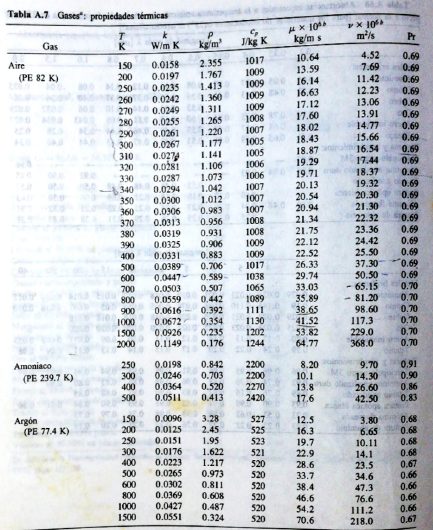
\includegraphics[width=1.2\textwidth]{Imagines/Propiedtermicasgases.png}
\caption{Propiedades térmicas del aire.[Tomado de \cite[p\ 868]{Mills}}]
\label{fig:propiedadesgases}
\end{figure}

\begin{figure}[H]
\centering
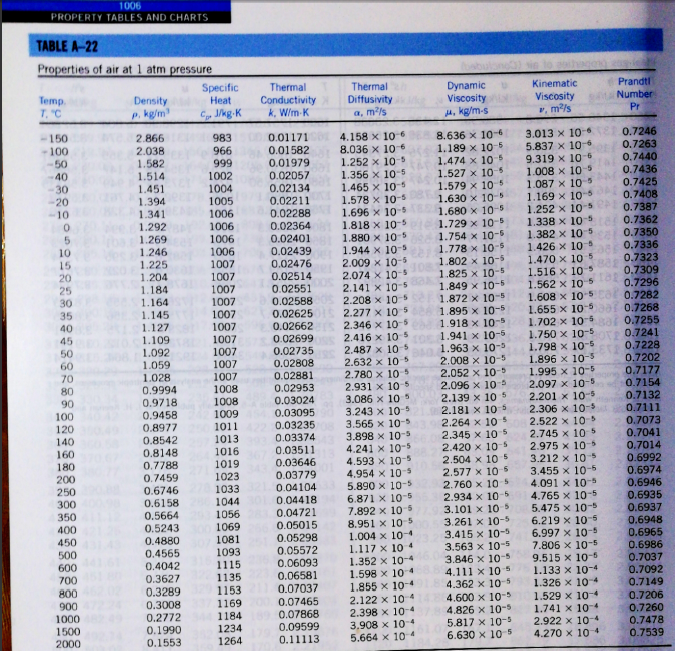
\includegraphics[width=1.2\textwidth]{Imagines/propaire1atm.png}
\caption{Propiedades del aire a 1 atm de presión .[Tomado de \cite[p\ 1006]{yunus}}
\label{fig:propiedadesaire}
\end{figure}



\begin{figure}[H]
\centering
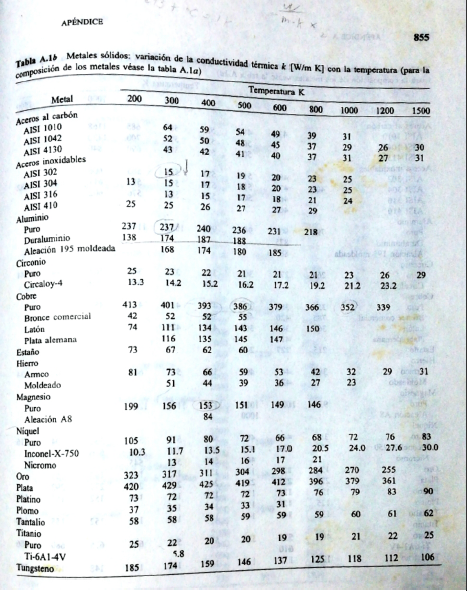
\includegraphics[width=1.2\textwidth]{Imagines/Varconductermicatemperatura.png}
\caption{ Variación de la conductividad térmica $k$ $[\frac{W}{mK}]$ en metales sólidos. Tomado de \cite[p\ 855]{Mills}}
\label{fig:conducciontermica}
\end{figure}

\begin{figure}[H]
\centering
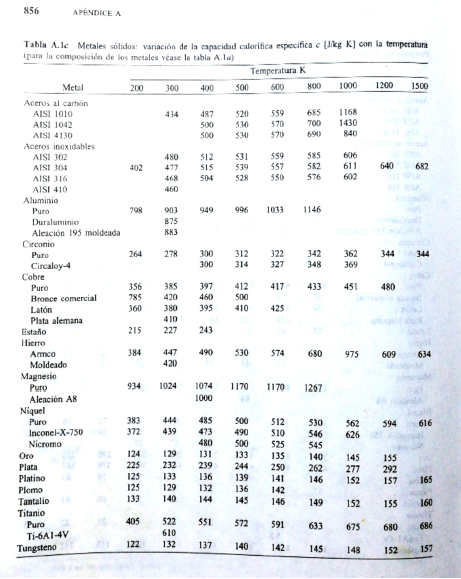
\includegraphics[width=1.2\textwidth]{Imagines/Varcapacalorifica.png}
\caption{Variación de la capacidad calorífica $c$ $[\frac{J}{KgK}]$ en metales sólidos. Tomado de \cite[p\ 856]{Mills}}
\label{fig:variacioncalorifica}
\end{figure}

\begin{figure}[H]
\centering
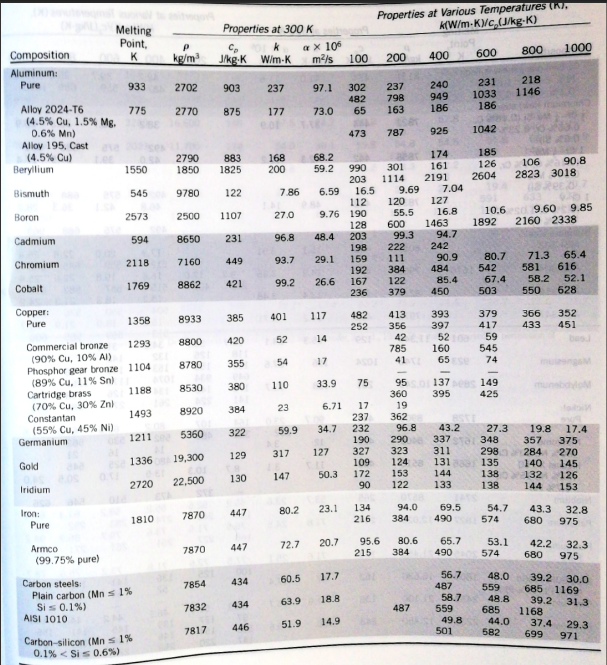
\includegraphics[width=1.2\textwidth]{Imagines/propiedadesmet1.png}
\caption{Propiedades de metales sólidos a diferentes temperaturas en Kelvin. Tomado de \cite[p\ 1009]{yunus}}
\label{fig:propiedadesmetales1}
\end{figure}

\begin{figure}[H]
\centering
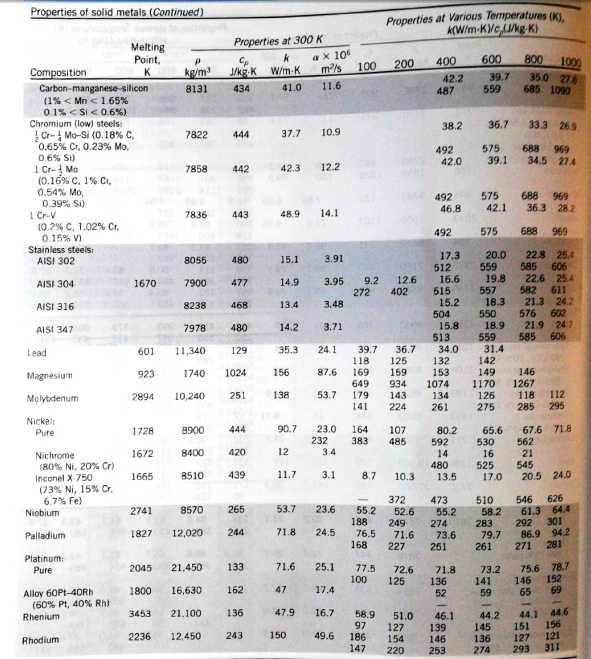
\includegraphics[width=1.2\textwidth]{Imagines/propiedadesmet2.png}
\caption{Propiedades de metales sólidos a diferentes temperaturas en Kelvin. Tomado de \cite[p\ 1010]{yunus}}
\label{fig:propiedadesmetales2}
\end{figure}



\newpage
\includepdf[pages=31-32]{PDF/thermophysical-properties.pdf}

\newpage
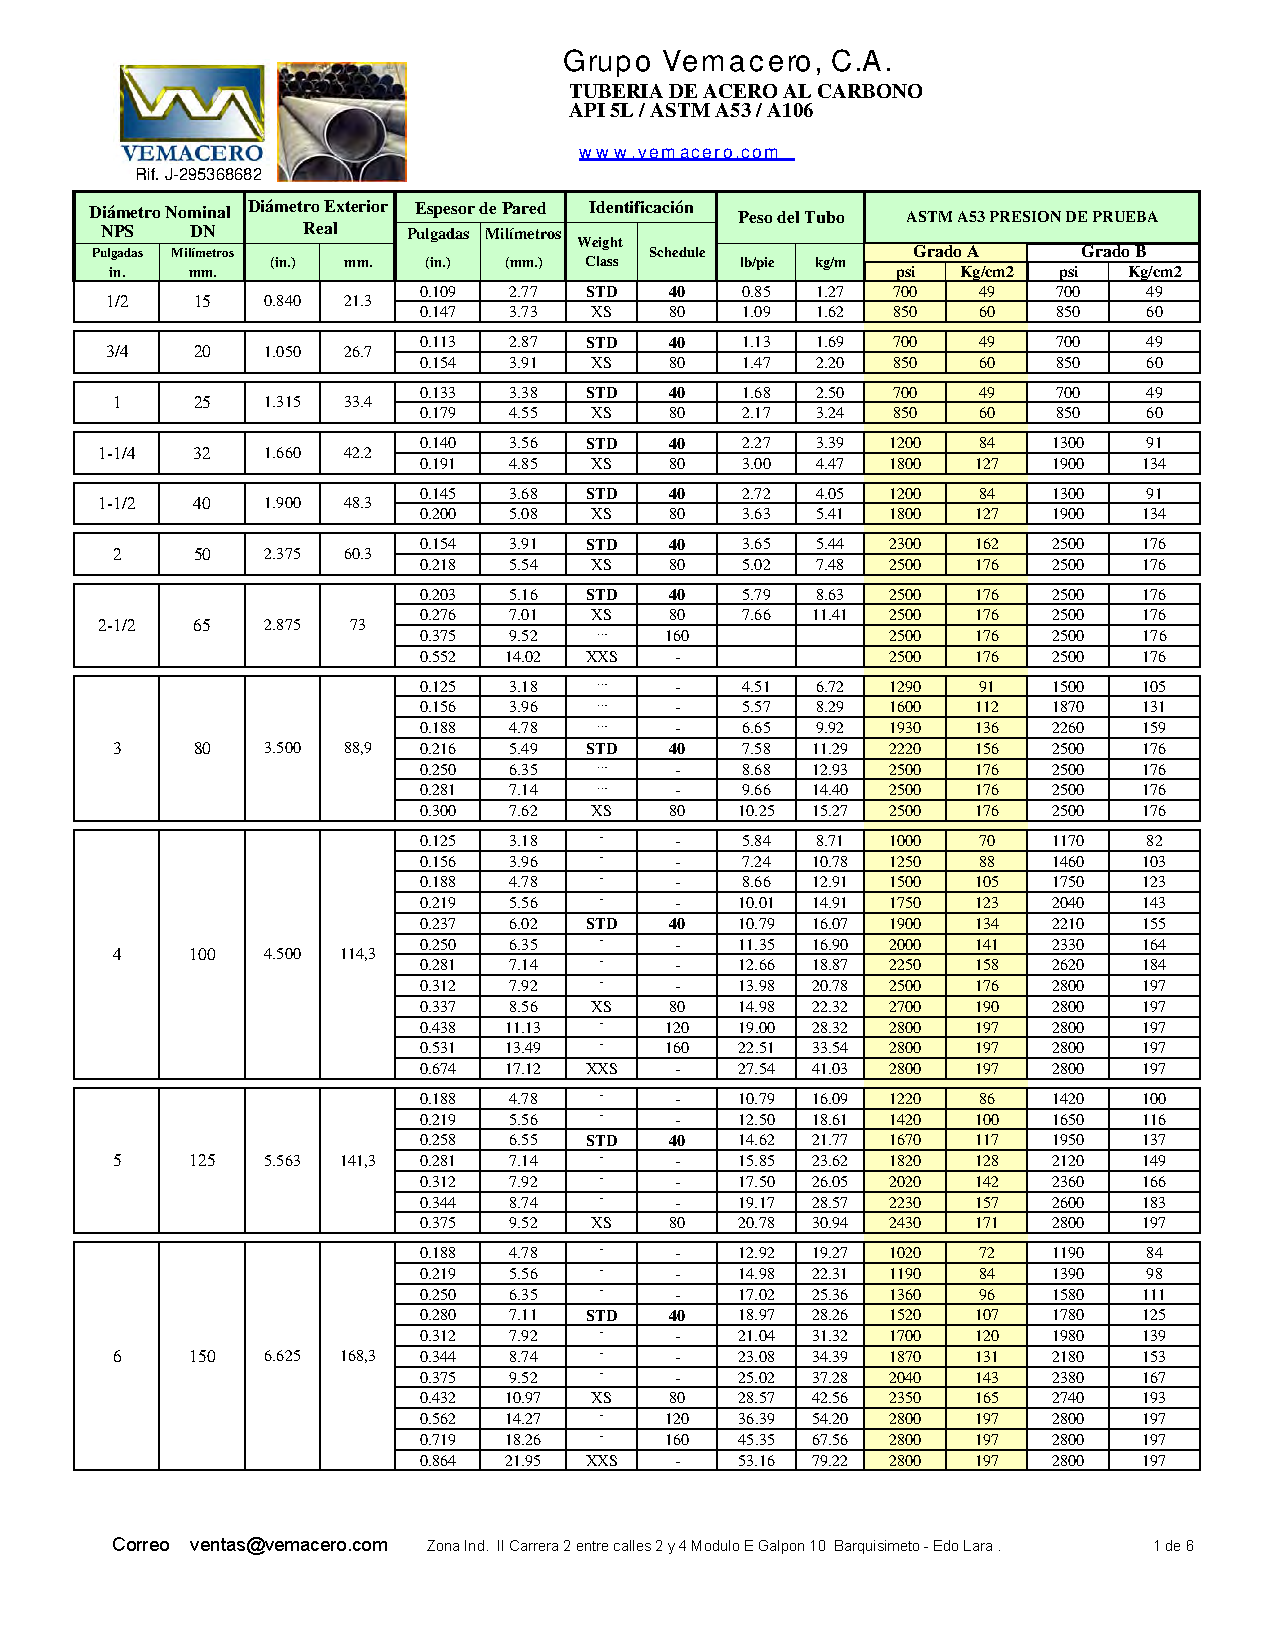
\includepdf[pages=1-3]{PDF/dimensionesdetuberiaaceroalcarbono.pdf}

\newpage
\includepdf[pages=79-84]{PDF/Disenomodulointercambiadorcalorcorazatubos}

\newpage
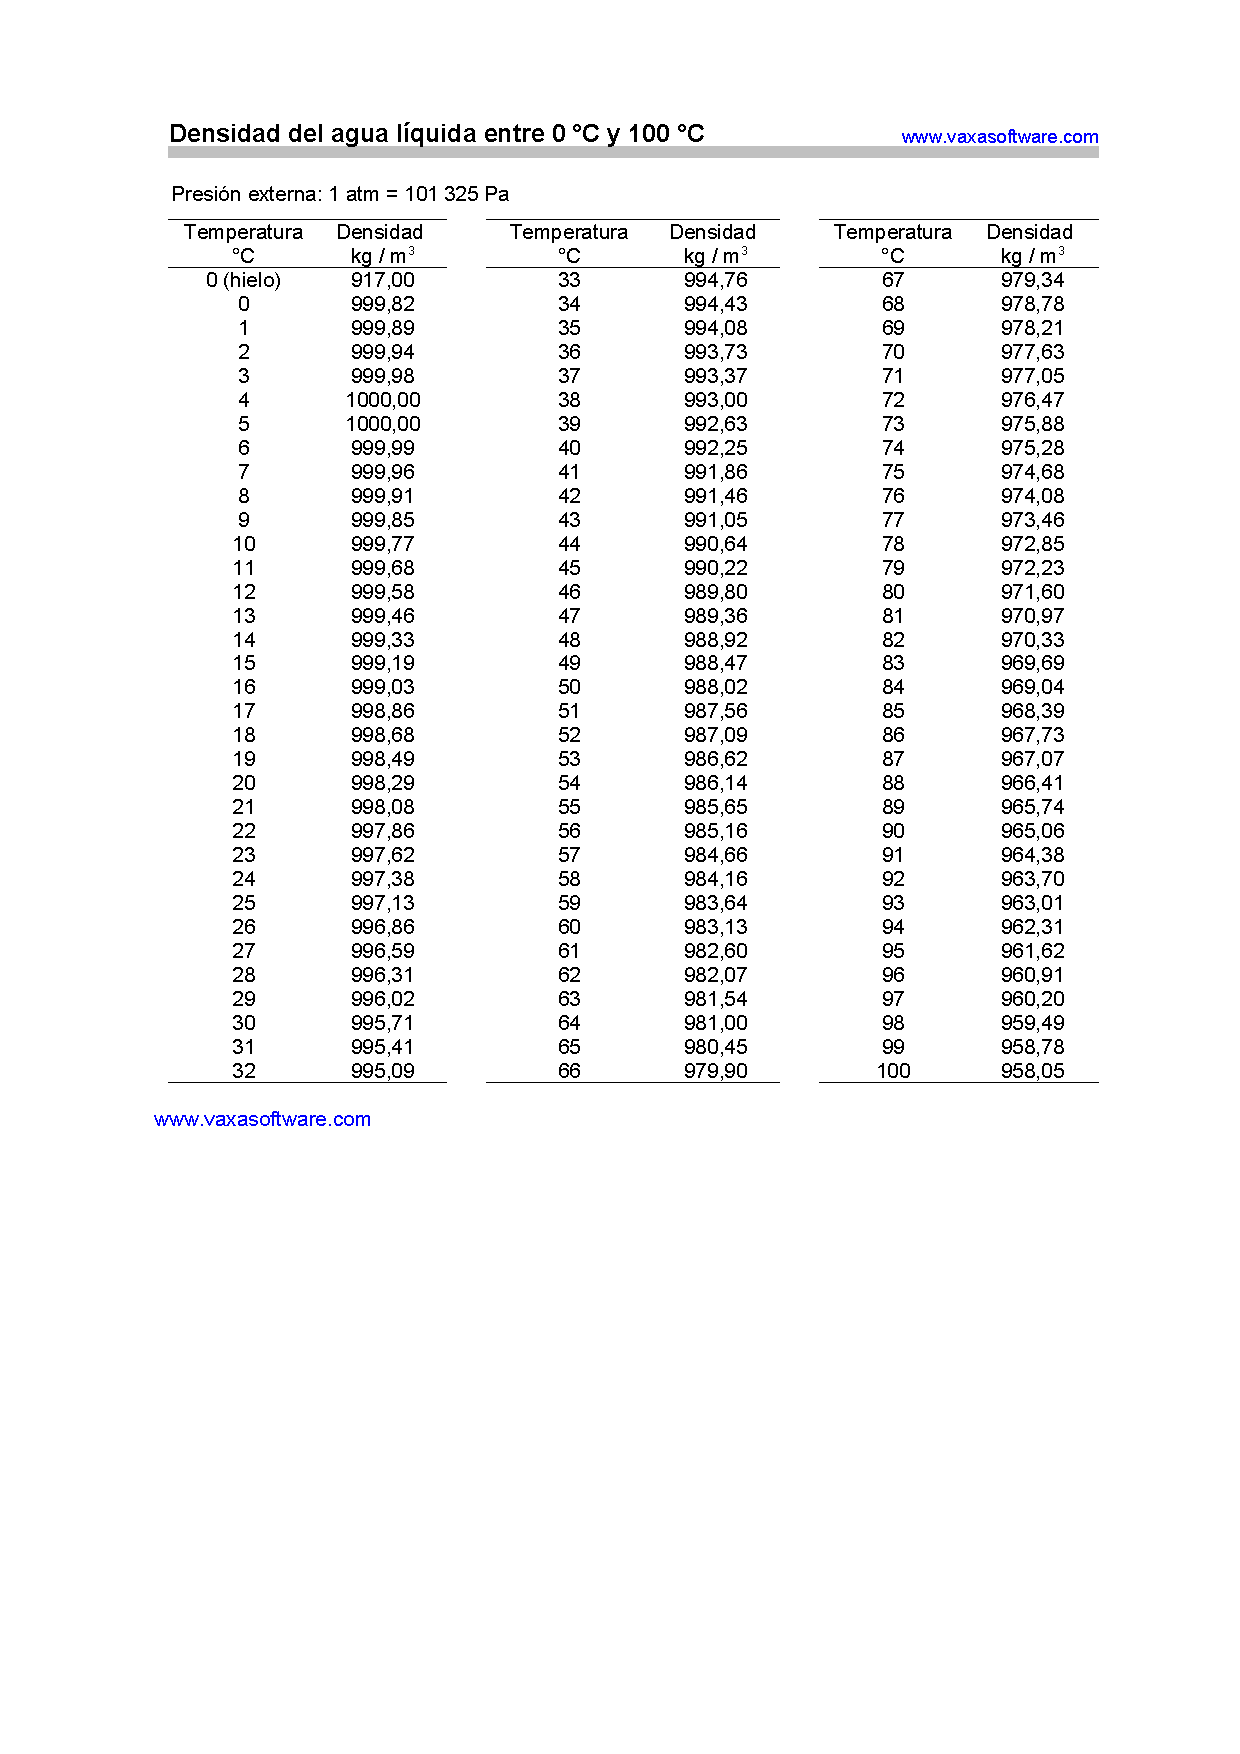
\includepdf[pages=-]{PDF/densidadaguadiferentestemperaturas.pdf}


\newpage
\begin{thebibliography}{}

\bibitem{Eduardo}
Cao Eduardo.(2010).\emph{Transfer in Process Engineering}.McGraw-Hill Education.Recuperado el 29 de Agosto de 2019.De https://www-accessengineeringlibrary-com.ezproxy.sibdi.ucr.ac.cr/content/book/9780071624084

\bibitem{Jaramillo}
Jaramillo. (2007). Intercambiadores de calor [Archivo PDF]. Recuperado de http://www.cie.unam.mx/~ojs/pub/HeatExchanger/Intercambiadores.pdf

\bibitem{Lopez}
Lopez Jose Costa. (1993). Curso de química técnica: introducción a los procesos, las operaciones unitarias y los fenómenos de transporte en la ingeniería química. Barcelona: Reverte.

\bibitem{Mills}
Mills,Anthony F.(1997).\emph{Transferencia de Calor}.University of California,Los Angeles.McGRAW-HLL. 

\bibitem{Natividad}
Natividad Rodríguez, Erik & Tovar León, Héctor (2014). Diseño de una planta virtual de un intercambiador de color en Matlab, con enlace al sistema de control FreeLancer. Instituto politécnico nacional, México.

\bibitem{Sadik}
Sadik,K.Hongtan, L.(1997).\emph{Heat Exchangers selection,rating and thermal design}.Department of Mechanical Engineering,University of Miami,Coral Gables,Florida.Editorial CRC Press.

\bibitem{Warren}
Warren M. Rohsenow; James P. Hartnett; Young I. Cho.(1998).\emph{Handbook of Heat Transfer}.McGraw-Hill Education: New York, Chicago, San Francisco, Athens, London, Madrid, Mexico City, Milan, New Delhi, Singapore, Sydney, Toronto.Recuperado el 29 de Agosto de 2019.De  https://www-accessengineeringlibrary-com.ezproxy.sibdi.ucr.ac.cr/content/book/9780070535558

\bibitem{Cengel}
 Yunus A. Cengel; (2007).\emph{Transferencia de calor y masa: un enfoque práctico}.McGraw-Hill Education
 
 \bibitem{yunus}
 Yunus A. Cengel; John M. Cimbala; Robert H. Tuner.(2012) \emph{Fundamentals of Thermal-fluid sciences}.New York. McGraw-Hill Education, fourth edition

\bibitem{Burbano}
Burbano Rojas,Sonia Paula .(2014).\emph{Diseño de un módulo de intercambiador de calor de coraza y tubos}.Universidad de Santo Tomás,
Facultad de ingeniería mecánica,
división de ingenierias,Bogota D.C.Recuperado el 25 de Octubre de 2019.De https://repository.usta.edu.co/bitstream/handle/11634/719/Diseno$\%20$de$\%20\%$un$\%20$modulo$\%20$de$\%20$intercambiador\%20$de$\%20$calor$\%20$de$\%20$coraza$\%20$y$\%20$tubos.pdf?sequence=1&isAllowed=y

\bibitem{vemacero}
Grupo Vemacero, C.A.\emph{TUBERIA DE ACERO AL CARBONO API 5L / ASTM A53 / A106}.Recuperado el 29 de Octubre de 2019.De https://www.vemacero.com/Tablas/A53MP.pdf

\end{thebibliography}{}


%%%%%%%%%%%%%%%%%%%%%%%%%%%%%%%%%%%%%%%%%%%%%%%%%%%%%%%%%%%%%%%%%

\end{document}